\documentclass{ldbc}

\usepackage{multirow}
\usepackage{float}
\usepackage{amsfonts}
\usepackage{bbding}
\usepackage{rotating}
\usepackage{pifont}
\usepackage{rotating}
\usepackage{subfigure}
\usepackage{amsmath}
\usepackage{longtable}
\usepackage{tabularx}
\usepackage{hyperref}
\usepackage{xspace}
\usepackage[table]{xcolor}
\usepackage{listings}
\providecommand{\tightlist}{%
	\setlength{\itemsep}{0pt}\setlength{\parskip}{0pt}}
\usepackage[export]{adjustbox}

\newcommand{\asc}{\uparrow}
\newcommand{\desc}{\downarrow}

\newcommand{\patternscale}{0.43}
\newcommand{\varname}[1]{\texttt{#1}}
\newcommand{\vartype}[1]{\footnotesize \textsf{#1}}
\newcommand{\variable}[2]{
	\renewcommand*{\arraystretch}{1}
	\begin{tabular}{|c|c|}\hline \varname{#1} & \cellcolor{gray!20} \vartype{#2}\\\hline\end{tabular}
	\renewcommand*{\arraystretch}{1.95}
}
\newcommand{\sortentry}[2]{
	\renewcommand*{\arraystretch}{1}
	\begin{tabular}{|c|c|}\hline \varname{#1} & $#2$\\\hline\end{tabular}
	\renewcommand*{\arraystretch}{1.95}
}
\newcommand{\chokepoint}[1]{\hyperref[choke_point_#1]{#1}}

\newcommand{\cmark}{\ding{51}}%
\newcommand{\xmark}{\ding{55}}%
\newcommand{\yes}{\color{green}\ding{51}\color{black}}
\newcommand{\no}{\color{red}\ding{55}\color{black}}

\newcommand{\cref}[1]{Chapter~\ref{#1}}
\newcommand{\sref}[1]{Section~\ref{#1}}
\newcommand{\tref}[1]{Table~\ref{#1}}
\newcommand{\fref}[1]{Figure~\ref{#1}}
\newcommand{\eref}[1]{Equation~\ref{#1}}
\newcommand{\aref}[1]{Appendix~\ref{#1}}

% Alex Averbuch: used internally only, to make missing/erroneous sections stand out
\newcommand{\alert}[1]{\textit{\textbf{{\color{red}#1}}}}

% todo change the following information as appropriate
%\WP{N/A}
\renewcommand{\wpIDText}{N/A}
\WPTitle{Social Network Benchmark Task Force}

%\delID{}
\renewcommand{\delIDText}{}
\delName{LDBC Social Network Benchmark (SNB) - v0.2.4 }

\dueDate{M12}
\submissionDate{M13}

%dissemination level
\dissPU % Public
%\dissRE % Restricted to group
%\dissPP % Restricted to programme
%\dissCO % Consortium-only

%nature
\natR % Report
%\natP % Prototype
%\natD % Demonstrator
%\natO % Other

%\author{[Arnau Prat (UPC)]}
%\authorPartner{Arnau Prat (UPC)}
%\responsibleAuthor{Arnau Prat}
%\responsiblePartner{UPC}
%\responsiblePhone{+34934054032}
%\responsibleEmail{aprat@ac.upc.edu}

% comment the following out if there are no contributors beside the main authors
%\contributor{[Peter Boncz (VUA), Josep Llu\'is Larriba (UPC), Renzo
%Angles (TALCA), Alex Averbuch (NEO), Orri Erling (OGL), Andrey
%Gubichev (TUM), Mirko Spasi\'c (OGL)], Minh-Duc Pham (VUA), Norbert Mart\'inez (SPARSITY)}

\reviewerOne{\alert{???}}
\reviewerTwo{\alert{???}}

\keywords{benchmark, choke points, dataset generator, graph database, query set, RDF, workload, auditing rules, publication rules, scale factors}

% for version numbers, use 2 digits separated by a dot (First digit is
% 0 for ``draft'', 1 for ``project approved'', 2 for ``further revisions''
% such as when the EC rejected version 1
\versionLog{
    \versionLogEntry{19/05/2014}{0.1}{Arnau Prat}{First draft}
}
\lastVersion{0.1}

% uncomment the following for final version
%\final

\documentUrl{\url{https://svn.sti2.at/ldbc/trunk/sib_spec/sib_spec.tex/}}
%\rhead{
\includegraphics[width=0.2\linewidth]{./figures/ldbc-logo.png}}

\abstract{
LDBC's Social Network Benchmark (\ldbcsnb) is an effort intended to test
various functionalities of systems used for graph-like data management. For this,
\ldbcsnb uses the recognizable scenario of operating a social network, characterized by
its graph-shaped data.

\ldbcsnb consists of two workloads that focus on different
functionalities: the interactive workload (interactive transactional queries)
and the business intelligence workload (analytical queries). 

This document contains the definition of the Interactive Workload and the first
draft of the Business Intelligence Workload. This includes a detailed
explanation of the data used in the \ldbcsnb benchmark, a detailed description
for all queries, and instructions on how to generate the data and run the
benchmark with the provided software.  
}


\execSummary{

The new data economy era, based on complexly structured, distributed and large
datasets, has brought on new demands on data management and analytics.  As a
consequence, new industry actors have appeared, offering technologies specially
built for the management of graph-like data. Also, traditional database
technologies, such as relational databases, are being adapted to the new
demands to remain competitive.

LDBC's Social Network Benchmark (\ldbcsnb) is an industrial and academic
initiative, formed by principal actors in the field of graph-like data
management. Its goal is to define a framework where different graph based
technologies can be fairly tested and compared, that can drive the
identification of systems' bottlenecks and required functionalities, and can
help researchers to open new research frontiers.

The philosophy around which \ldbcsnb is designed is to be easy to
understand, flexible and cheap to adopt. For all these reasons,
\ldbcsnb will propose different workloads representing all the usage scenarios
of graph-like database technologies, hence, targeting systems of different
nature and characteristics.  In order increase its adoption by industry and
research institutions, \ldbcsnb provides all necessary software, which are
designed to be easy to use and deploy at a small cost.

This document contains:
\begin{itemize}
\item A detailed specification of the data used in the whole \ldbcsnb benchmark.
\item A detailed specification of the workloads.
\item A detailed specification of the execution rules of the benchmark.
\item A detailed specification of the auditing rules and the full disclosure
  report's required contents.
\end{itemize}
}


\begin{document}

\maketitle

%\include{glossary}

\chapter*{Special thanks}
Special thanks to all the people that have contributed to the development of
this benchmark:
\begin{itemize}
  \item Renzo Angles (Universidad de Talca)
  \item Alex Averbuch (Neo Technologies)
  \item Peter Boncz (Vrije Universiteit Amsterdam)
  \item Orri Erling (Google)
  \item Andrey Gubichev (Google)
  \item Moritz Kaufmann (Technische Universit\"at M\"unchen)
  \item Josep Llu\'is Larriba Pey (Universitat Polit\`ecnica de Catalunya)
  \item Minh-Duc Pham (Altran)
  \item Marcus Paradies (SAP)
  \item Arnau Prat (Sparsity Technologies)
  \item Mirko Spasi\'c (Openlink Software)
  \item Norbert Mart\'inez (Huawei Technologies)
\end{itemize}

\listoffigures
\listoftables
\chapter*{Definitions}
\chapter*{Definitions}

%{\flushleft \textbf{ACID}}: The transactional properties of Atomicity,
%Consistency, Isolation and Durability.
%
%
%{\flushleft \textbf{Commit:}} a control operation that:
%        \begin{itemize}
%            \item Is initiated by a unit of work (a Transaction) 
%            \item Is implemented by the DBMS 
%            \item Signifies that the unit of work has completed successfully
%and all tentatively modified data are to persist (until modified by some other
%operation or unit of work) 
 Upon successful completion of this control
%operation both the Transaction and the data are said to be Committed. 
%        \end{itemize}
%
%
%{\flushleft \textbf{DBMS:}} A Data Base Management System is a collection
%of programs that enable you to store, modify, and extract information from a
%database.
%
%
%
%{\flushleft \textbf{Durability:}} In general, state that persists
%across failures is said to be Durable and an implementation that ensures state
%persists across failures is said to provide Durability. In the context of the
%benchmark, Durability is more tightly defined as the SUT‘s ability to ensure
%all Committed data persist across any Single Point of Failure.
%
%{\flushleft \textbf{Measurement Window:}} This is the time window when the
%benchmark records statistics. It must fulfill the requirements defined in 
%\alert{Section XX}.
%
%{\flushleft \textbf{Performance Metric:}} The \ldbcsnb Reported Throughput as
%expressed in tps. This is known as the Performance Metric.
%
%{\flushleft \textbf{Price/Performance Metric:}} The \ldbcsnb total 3-year
%pricing divided by the Reported Throughput is price/tpsE. This is also known as
%the Price/Performance Metric.


{\flushleft \textbf{\datagen:}} Is the data generator provided by the \ldbcsnb, which
is responsible for generating the data needed to run the benchmark.

{\flushleft \textbf{DBMS:}} A DataBase Management System. 

{\flushleft \textbf{\ldbcsnb:}} Linked Data Benchmark Council Social Network Benchmark. 

{\flushleft \textbf{Query Mix:}} Refers to the ratio between read and update queries
of a workload, and the frequency at which they are issued.

{\flushleft \textbf{SF (Scale Factor):}} The \ldbcsnb is designed to target systems of
different size and scale. The scale factor determines the size of the data used
to run the benchmark, measured in Gigabytes.


{\flushleft \textbf{SUT:}} The System Under Test  is defined
to be the database system where the benchmark is executed.


{\flushleft \textbf{Test Driver:}}  A program provided by the \ldbcsnb, which
is responsible for executing the different workloads and gathering the results.

{\flushleft \textbf{Test Sponsor:}} The Test Sponsor is the company officially
submitting the Result with the FDR and will be charged the filing fee. Although
multiple companies may sponsor a Result together, for the purposes of the LDBC
processes the Test Sponsor must be a single company. A Test Sponsor need not be
a LDBC member. The Test Sponsor is responsible for maintaining the FDR with any
necessary updates or corrections. The Test Sponsor is also the name used to
identify the Result.

%{\flushleft \textbf{Test Run:}} The entire period of time during which Drivers
%submit and the SUT completes Transactions other than Trade-Cleanup.
%
%{\flushleft \textbf{Transaction:}} 
A Database Transaction is an ACID unit of work.


%{\flushleft \textbf{Valid Transaction:}} The term Valid Transaction refers to
%any Transaction for which input data has been sent in full by the Driver, whose
%processing has been successfully completed on the SUT and whose correct output
%data has been received in full by the Driver.

{\flushleft \textbf{Workload:}} A workload refers to a set of queries of a given nature
(\ie interactive, analytical, business), how they are issued and at which rate.


\chapter{Introduction}
\chapter{Introduction}
\label{section:introduction}

%%%%%%%%%%%%%%%%%%%%%%%%%%%%%%%%%%%%%%%%%%%%%%%%%%%%%%%%%%%%%%%%%%%%%%%%%%%%%%
%%%%%%%%%%%%%%%%%%%%%%%%%%%%%%%%%%%%%%%%%%%%%%%%%%%%%%%%%%%%%%%%%%%%%%%%%%%%%%
%%%%%%%%%%%%%%%%%%%%%%%%%%%%%%%%%%%%%%%%%%%%%%%%%%%%%%%%%%%%%%%%%%%%%%%%%%%%%%

\section{Motivation for the Benchmark}

The new era of data economy, based on large, distributed, and complexly
structured data sets, has brought on new and complex challenges in the field of
data management and analytics. These data sets, usually modeled as large
graphs, have attracted both industry and academia, due to new
opportunities in research and innovation they offer. This situation has also
opened the door for new companies to emerge, offering new non-relational and
graph-like technologies that are called to play a significant role in upcoming
years.

The change in the data paradigm calls for new benchmarks to test these new
emerging technologies, as they set a framework where different systems can
compete and be compared in a fair way, they let technology providers identify
the bottlenecks and gaps of their systems and, in general, drive the research
and development of new information technology solutions. Without them, the
uptake of these technologies is at risk by not providing the industry with
clear, user-driven targets for performance and functionality.

The LDBC Social Network Benchmark (\ldbcsnb) aims at being a comprehensive
benchmark by setting the rules for the evaluation of graph-like data management
technologies.  \ldbcsnb is designed to be a plausible look-alike of all the
aspects of operating a social network site, as one of the most representative
and relevant use cases of modern graph-like applications.

\ldbcsnb includes the Interactive
Workload~\cite{DBLP:conf/sigmod/ErlingALCGPPB15}, which consists of user-centric
transactional-like interactive queries, and the Business Intelligence Workload,
which includes analytic queries to respond to business-critical questions.
Initially, a graph analytics workload was also included in the roadmap of
\ldbcsnb, but this was finally delegated to the Graphalytics benchmark
project~\cite{DBLP:journals/pvldb/IosupHNHPMCCSAT16}, which was adopted as an official LDBC graph
analytics benchmark. \ldbcsnb and Graphalytics combined target a broad range of
systems with different nature and characteristics.  \ldbcsnb and Graphalytics
aim at capturing the essential features of these scenarios while
abstracting away details of specific business deployments.

This document contains the definition of the Interactive Workload and the first
draft of the Business Intelligence Workload. This includes a detailed
explanation of the data used in the \ldbcsnb benchmark, a detailed description
for all queries, and instructions on how to generate the data and run the
benchmark with the provided software.

%%%%%%%%%%%%%%%%%%%%%%%%%%%%%%%%%%%%%%%%%%%%%%%%%%%%%%%%%%%%%%%%%%%%%%%%%%%%%%
%%%%%%%%%%%%%%%%%%%%%%%%%%%%%%%%%%%%%%%%%%%%%%%%%%%%%%%%%%%%%%%%%%%%%%%%%%%%%%
%%%%%%%%%%%%%%%%%%%%%%%%%%%%%%%%%%%%%%%%%%%%%%%%%%%%%%%%%%%%%%%%%%%%%%%%%%%%%%

\section{Relevance to the Industry}

\ldbcsnb is intended to provide the following value to different stakeholders:

\begin{itemize}
 \item For \textbf{end users} facing graph processing tasks, \ldbcsnb provides
     a recognizable scenario against which it is possible to compare merits of
     different products and technologies.  By covering a wide variety of scales
     and price points, \ldbcsnb can serve as an aid to technology selection.
 \item For \textbf{vendors} of graph database technology, \ldbcsnb provides a
     checklist of features and performance characteristics that helps in
     product positioning and can serve to guide new development.
 \item For \textbf{researchers}, both industrial and academic, the \ldbcsnb
     dataset and workload provide interesting challenges in multiple
     choke point areas, such as query optimization, (distributed) graph
     analysis, transactional throughput, and provides a way to objectively
     compare the effectiveness and efficiency of new and existing technology in
     these areas.
\end{itemize}

The technological scope of \ldbcsnb comprises all systems that one might
conceivably use to perform social network data management tasks:

\begin{itemize}
 \item \textbf{Graph database systems} (\eg Neo4j, InfiniteGraph, Sparksee,
     Titan/JanusGraph) are novel technologies aimed at storing directed and labeled
     graphs. They support graph traverals, typically by means of APIs, though
     some of them also support dedicated graph-oriented query languages (\eg
     Neo4j's Cypher). These systems' internal structures are typically designed
     to store dynamic graphs that change over time.  They offer support for
     transactional queries with some degree of consistency, and value-based
     indexes to quickly locate nodes and edges. Finally, their architecture is
     typically single-machine (non-cluster). These systems can
     potentially implement all three workloads, though Interactive and Business Intelligence
     workloads are where they will presumably be more competitive.
 \item \textbf{Graph processing frameworks} (\eg Giraph, Signal/Collect,
     GraphLab, Green Marl) are designed to perform global graph
     computations, executed in parallel or in a lockstep fashion. These computations are typically
     long latency, involving many nodes and edges and often consist of approximation
     answers to NP-complete problems. These systems expose an API, sometimes following
     a vertex-centric paradigm, and their architecture targets both single-machine and
     cluster systems. These systems will likely implement the Graph Analytics workload.
 \item \textbf{RDF database systems} (\eg OWLIM, Virtuoso, BigData, Jena TDB,
     Stardog, Allegrograph) are systems that implement the SPARQL~1.1 query
     language, similar in complexity to \mbox{SQL-92}, which allows for structured
     queries, and simple traversals. RDF database systems often come with
     additional support for simple reasoning (sameAs, subClass), text search, and
     geospatial predicates.  RDF database systems generally support
     transactions, but not always with full concurrency and serializability and
     their supposed strength is integrating multiple data sources (\eg
     DBpedia). Their architecture is both single-machine and clustered, and
     they will likely target Interactive and Business Intelligence workloads.
\item \textbf{Relational database systems} (\eg Postgres, MySQL, Oracle, IBM DB2,
     Microsoft SQL Server, Virtuoso, MonetDB, Vectorwise, Vertica, but also Hive and
     Impala) treat graph data relationally, and queries are formulated in SQL and/or
     PL/SQL. Both single-machine and cluster systems exist. They do not
     normally support recursion or stateful recursive algorithms, which makes     them not at home in the Graph Analytics workloads.
 \item \textbf{NoSQL database systems} (\eg key-value stores such as HBase,
     REDIS, MongoDB, CouchDB, or even MapReduce systems like Hadoop and Pig)
     are cluster-based and scalable. Key-value stores could possibly implement
     the Interactive Workload, though its navigational aspects would pose some
     problems as potentially many key-value lookups are needed. MapReduce
     systems could be suited for the Graph Analytics workload, but their query
     latency would presumably be so high that the Business Intelligence
     workload would not make sense, though we note that some of the key-value
     stores (\eg MongoDB) provide a MapReduce query functionality on the data
     that it stores which could make it suited for the Business Intelligence workload.
\end{itemize}

%%%%%%%%%%%%%%%%%%%%%%%%%%%%%%%%%%%%%%%%%%%%%%%%%%%%%%%%%%%%%%%%%%%%%%%%%%%%%%
%%%%%%%%%%%%%%%%%%%%%%%%%%%%%%%%%%%%%%%%%%%%%%%%%%%%%%%%%%%%%%%%%%%%%%%%%%%%%%
%%%%%%%%%%%%%%%%%%%%%%%%%%%%%%%%%%%%%%%%%%%%%%%%%%%%%%%%%%%%%%%%%%%%%%%%%%%%%%

\section{General Benchmark Overview}

\ldbcsnb aims at being a complete benchmark, designed with the following goals in mind:

\begin{itemize}
 \item \textbf{Rich coverage}. \ldbcsnb is intended to cover most demands
     encountered in the management of complexly structured data.
 \item \textbf{Modularity}. \ldbcsnb is broken into parts that can be
     individually addressed. In this manner \ldbcsnb
     stimulates innovation without imposing an overly high threshold for
     participation.
 \item \textbf{Reasonable implementation cost}. For a product offering relevant
     functionality, the effort for obtaining initial results with SNB should be
     small, in the order of days.
 \item \textbf{Relevant selection of challenges}. Benchmarks are known to
     direct product development in certain directions. \ldbcsnb is informed by
     the state-of-the-art in database research so as to offer optimization
     challenges for years to come while not having a prohibitively high
     threshold for entry.
 \item \textbf{Reproducibility and documentation of results}. \ldbcsnb
     will specify the rules for full disclosure of benchmark execution and for
     auditing of benchmark runs. The workloads may be run on any equipment
     but the exact configuration and price of the hardware and software must be
     disclosed.
\end{itemize}

\ldbcsnb benchmark is modeled around the operation of a real social network
site. A social network site represents a relevant use case for the following
reasons:

\begin{itemize}
    \item It is simple to understand for a large audience, as it is
        arguably present in our every-day life in different shapes and forms.
    \item It allows testing a complete range of interesting
        challenges, by means of different workloads targeting systems of
        different nature and characteristics.
    \item A social network can be scaled, allowing the design of a
        scalable benchmark targeting systems of different sizes and budgets.
\end{itemize}

In \autoref{section:data}, \ldbcsnb defines the schema of the data used in
the benchmark. The schema represents a realistic social network, including
people and their activities in the social network during a period of time.
Personal information of each person, such as name, birthday, interests
or places where people work or study, is included. A persons' activity is
represented in the form of friendship relationships and content sharing (\ie
messages and pictures). \ldbcsnb provides a scalable synthetic data generator
based on the MapReduce paradigm, which produces networks with the
described schema with distributions and correlations similar to those expected
in a real social network. Furthermore, the data generator is designed to be
user-friendly. The proposed data schema is shared by all the different proposed
workloads, those we currently have, and those that will be proposed in the future.

In \autoref{section:workloads}, the Interactive Workload and the first draft of
the Business Intelligence workload are proposed. Workloads are designed to mimic
the different usage scenarios found in operating a real social network site, and
each of them targets one or more types of systems.  Each workload defines a set
of queries and query mixes, designed to stress the SUTs in different choke point
areas, while being credible and realistic. The Interactive workload reproduces the
interaction between the users of the social network by including lookups and
transactions, which update small portions of the database. These queries are
designed to be interactive and target systems capable of responding to such queries
with low latency for multiple concurrent users. The Business Intelligence workload
represents analytic queries a social network company would
like to perform in the social network, to take advantage of the data and to
discover new business opportunities. This workload explores moderate to large
portions of the graph from different entities, and performs more resource-intensive
operations.

\ldbcsnb provides an execution test driver, which is responsible for executing
the workloads and gathering the results. The driver is designed with simplicity
and portability in mind to ease the implementation on systems with different
nature and characteristics at a low implementation cost. Furthermore, it
automatically handles the validation of the queries by means of a validation
dataset provided by LDBC.  The overall philosophy of \ldbcsnb is to provide
the necessary software tools to run the benchmark, and therefore to reduce the
benchmark's entry point as much as possible.

%%%%%%%%%%%%%%%%%%%%%%%%%%%%%%%%%%%%%%%%%%%%%%%%%%%%%%%%%%%%%%%%%%%%%%%%%%%%%%
%%%%%%%%%%%%%%%%%%%%%%%%%%%%%%%%%%%%%%%%%%%%%%%%%%%%%%%%%%%%%%%%%%%%%%%%%%%%%%
%%%%%%%%%%%%%%%%%%%%%%%%%%%%%%%%%%%%%%%%%%%%%%%%%%%%%%%%%%%%%%%%%%%%%%%%%%%%%%

\section{Related Projects}

Along the Social Network Benchmark, LDBC~\cite{DBLP:journals/sigmod/AnglesBLF0ENMKT14} provides other benchmarks as well:

\begin{itemize}
	\item The Semantic Publishing Benchmark (SPB)~\cite{DBLP:conf/semweb/SpasicJP16} measures the performance of \emph{semantic databases} operating on RDF data sets.
	\item The Graphalytics benchmark~\cite{DBLP:journals/pvldb/IosupHNHPMCCSAT16} measures the performance of \emph{graph analysis} operations (\eg PageRank, local clustering coefficient).
\end{itemize}

%%%%%%%%%%%%%%%%%%%%%%%%%%%%%%%%%%%%%%%%%%%%%%%%%%%%%%%%%%%%%%%%%%%%%%%%%%%%%%
%%%%%%%%%%%%%%%%%%%%%%%%%%%%%%%%%%%%%%%%%%%%%%%%%%%%%%%%%%%%%%%%%%%%%%%%%%%%%%
%%%%%%%%%%%%%%%%%%%%%%%%%%%%%%%%%%%%%%%%%%%%%%%%%%%%%%%%%%%%%%%%%%%%%%%%%%%%%%

\section{Participation of Industry and Academia}

The list of institutions that take part in the definition and development
of \ldbcsnb is formed by relevant actors from both the industry and academia in
the field of linked data management. All the participants have contributed with
their experience and expertise in the field, making a credible and relevant
benchmark, which meets all the desired needs. The list of participants is the
following:

\begin{itemize}
    \item FOUNDATION FOR RESEARCH AND TECHNOLOGY HELLAS
    \item MTA-BME LENDUELET RESEARCH GROUP ON CYBER-PHYSICAL SYSTEMS
    \item NEO4J
    \item ONTOTEXT
    \item OPENLINK
    \item TECHNISCHE UNIVERSITAET MUENCHEN
    \item UNIVERSITAET INNSBRUCK
    \item UNIVERSITAT POLITECNICA DE CATALUNYA
    \item VRIJE UNIVERSITEIT AMSTERDAM
\end{itemize}

\begin{figure}
\end{figure}

Besides the aforementioned institutions, during the development of the
benchmark several meetings with the technical and users community have been
conducted, receiving an invaluable feedback that has contributed to the whole
development of the benchmark in every of its aspects.

%%%%%%%%%%%%%%%%%%%%%%%%%%%%%%%%%%%%%%%%%%%%%%%%%%%%%%%%%%%%%%%%%%%%%%%%%%%%%%
%%%%%%%%%%%%%%%%%%%%%%%%%%%%%%%%%%%%%%%%%%%%%%%%%%%%%%%%%%%%%%%%%%%%%%%%%%%%%%
%%%%%%%%%%%%%%%%%%%%%%%%%%%%%%%%%%%%%%%%%%%%%%%%%%%%%%%%%%%%%%%%%%%%%%%%%%%%%%


\chapter{Benchmark Specification}
%%% FORMAL DEFINITION %%%

%%%%%%%%%%%%%%%%%%%%%%%%%%%%%%%%%%%%%%%%%%%%%%%%%%%%%%%%%%%%%%%%%%%%%%%%%%%%%%
%%%%%%%%%%%%%%%%%%%%%%%%%%%%%%%%%%%%%%%%%%%%%%%%%%%%%%%%%%%%%%%%%%%%%%%%%%%%%%
%%%%%%%%%%%%%%%%%%%%%%%%%%%%%%%%%%%%%%%%%%%%%%%%%%%%%%%%%%%%%%%%%%%%%%%%%%%%%%

\section{Requirements}

LDBC-SNB is designed to be flexible and to have an affordable entry point.
From small single node and in memory systems to large distributed multi-node
clusters have its own place in LDBC-SNB.  Therefore, the requirements to
fulfill for executing LDBC-SNB are limited to pure software requirements to be
able to run the tools. All the software provided by LDBC-SNB have been
developed and tested under Linux-based operating systems.

LDBC-SNB does not impose the usage of any specific type of system, as it
targets systems of different nature and characteristics, from graph databases,
graph processing frameworks and RDF systems, to traditional relational database
management systems. Consequently, any language or API capable of expressing the
proposed queries can be used. Similarly, data can be stored in the most
convenient manner the test sponsor may decide.

%, as long as it conforms with the
%execution rules. Finally, in order to have an official benchmark execution, the
%results will have to be audited and all the required information disclosed.

\section{Software and Useful links} 

\begin{itemize}
    \item \textbf{LDBC Driver 0.3 -- \url{https://github.com/ldbc/ldbc_driver}}: The driver
    responsible for executing the LDBC-SNB workload.
    \item \textbf{DATAGEN 0.2.5 -- \url{https://github.com/ldbc/ldbc_snb_datagen}}: The data
    generator used to generate the datasets of the benchmark.
\end{itemize}
%%%%%%%%%%%%%%%%%%%%%%%%%%%%%%%%%%%%%%%%%%%%%%%%%%%%%%%%%%%%%%%%%%%%%%%%%%%%%%
%%%%%%%%%%%%%%%%%%%%%%%%%%%%%%%%%%%%%%%%%%%%%%%%%%%%%%%%%%%%%%%%%%%%%%%%%%%%%%
%%%%%%%%%%%%%%%%%%%%%%%%%%%%%%%%%%%%%%%%%%%%%%%%%%%%%%%%%%%%%%%%%%%%%%%%%%%%%%
%%%%%%%%%%%%%%%%%%%%%%%%%%%%%%%%%%%%%%%%%%%%%%%%%%%%%%%%%%%%%%%%%%%%%%%%%%%%%%
%%%%%%%%%%%%%%%%%%%%%%%%%%%%%%%%%%%%%%%%%%%%%%%%%%%%%%%%%%%%%%%%%%%%%%%%%%%%%%
%%%%%%%%%%%%%%%%%%%%%%%%%%%%%%%%%%%%%%%%%%%%%%%%%%%%%%%%%%%%%%%%%%%%%%%%%%%%%%

\section{Data}\label{section:data}

This section introduces the data used by LDBC-SNB. This includes the different
data types, the data schema, how it is generated and the different scale
factors.

\subsection{Data Types}
Table~\ref{table:types} describes the different types used in the whole benchmark.

\begin{table}[h]
\centering
\begin{tabular}{|p{2.5cm}|p{13cm}|}
    \hline
    \textbf{Type} & \textbf{Description} \\
    \hline
    ID &  integer type with 64-bit precision. All IDs within a single entity are unique\\
    \hline
    32-bit Integer &  integer type with 32-bit precision\\
    \hline
    64-bit Integer &  integer type with 64-bit precision\\
    \hline
    String & variable length text of size 40 Unicode characters\\
    \hline
    Long String & variable length text of size 256 Unicode characters\\
    \hline
    Text &  variable length text of size 2000 Unicode characters\\
    \hline
    Date &  date with a precision of a day, encoded as a string with the following format: \textit{yyyy-mm-dd}, where \textit{yyyy} is a four-digit integer representing the year,
    the year, \textit{mm} is a two-digit integer representing the month and dd is a two-digit integer representing the day. \\
    \hline
    DateTime &  date with a precision of milliseconds, encoded as a string with the following format: \textit{yyyy-mm-ddTHH:MM:ss.sss+0000}, where \textit{yyyy} is a four-digit integer representing the year,
    the year, \textit{mm} is a two-digit integer representing the month and \textit{dd} is a two-digit integer representing the day, \textit{HH} is a two-digit integer representing the hour, \textit{MM} is a two
    digit integer representing the minute and \textit{ss.sss} is a five digit fixed point real number representing the seconds up to millisecond precision. Finally, the \textit{+0000} of the end represents the
    timezone, which in this case is always GMT.\\
    \hline
\end{tabular}
\caption{Description of the data types.}
\label{table:types}
\end{table}


\subsection{Data Schema}

Figure~\ref{figure:schema} shows the data schema in UML. The schema defines the
structure of the data used in the benchmark in terms of entities and their
relations. Data represents a snapshot of the activity of a social network
during a period of time. Data includes entities such as Persons, Organizations,
and Places. The schema also models the way persons interact, by means of the
friendship relations established with other persons, and the sharing of content
such as messages (both textual and images), replies to messages and likes to
messages.  People form groups to talk about specific topics, which are
represented as tags.

LDBC-SNB has been designed to be flexible and to target systems of different
nature and characteristics. As such, it does not force any particular internal
representation of the schema. The DATAGEN component
% described in Section~\ref{section:data_generation}
supports multiple output data formats to
fit the needs of different types of systems, including RDF, relational DBMS and
graph DBMS.

%\begin{landscape}
%    \begin{figure}
%        \centering
%        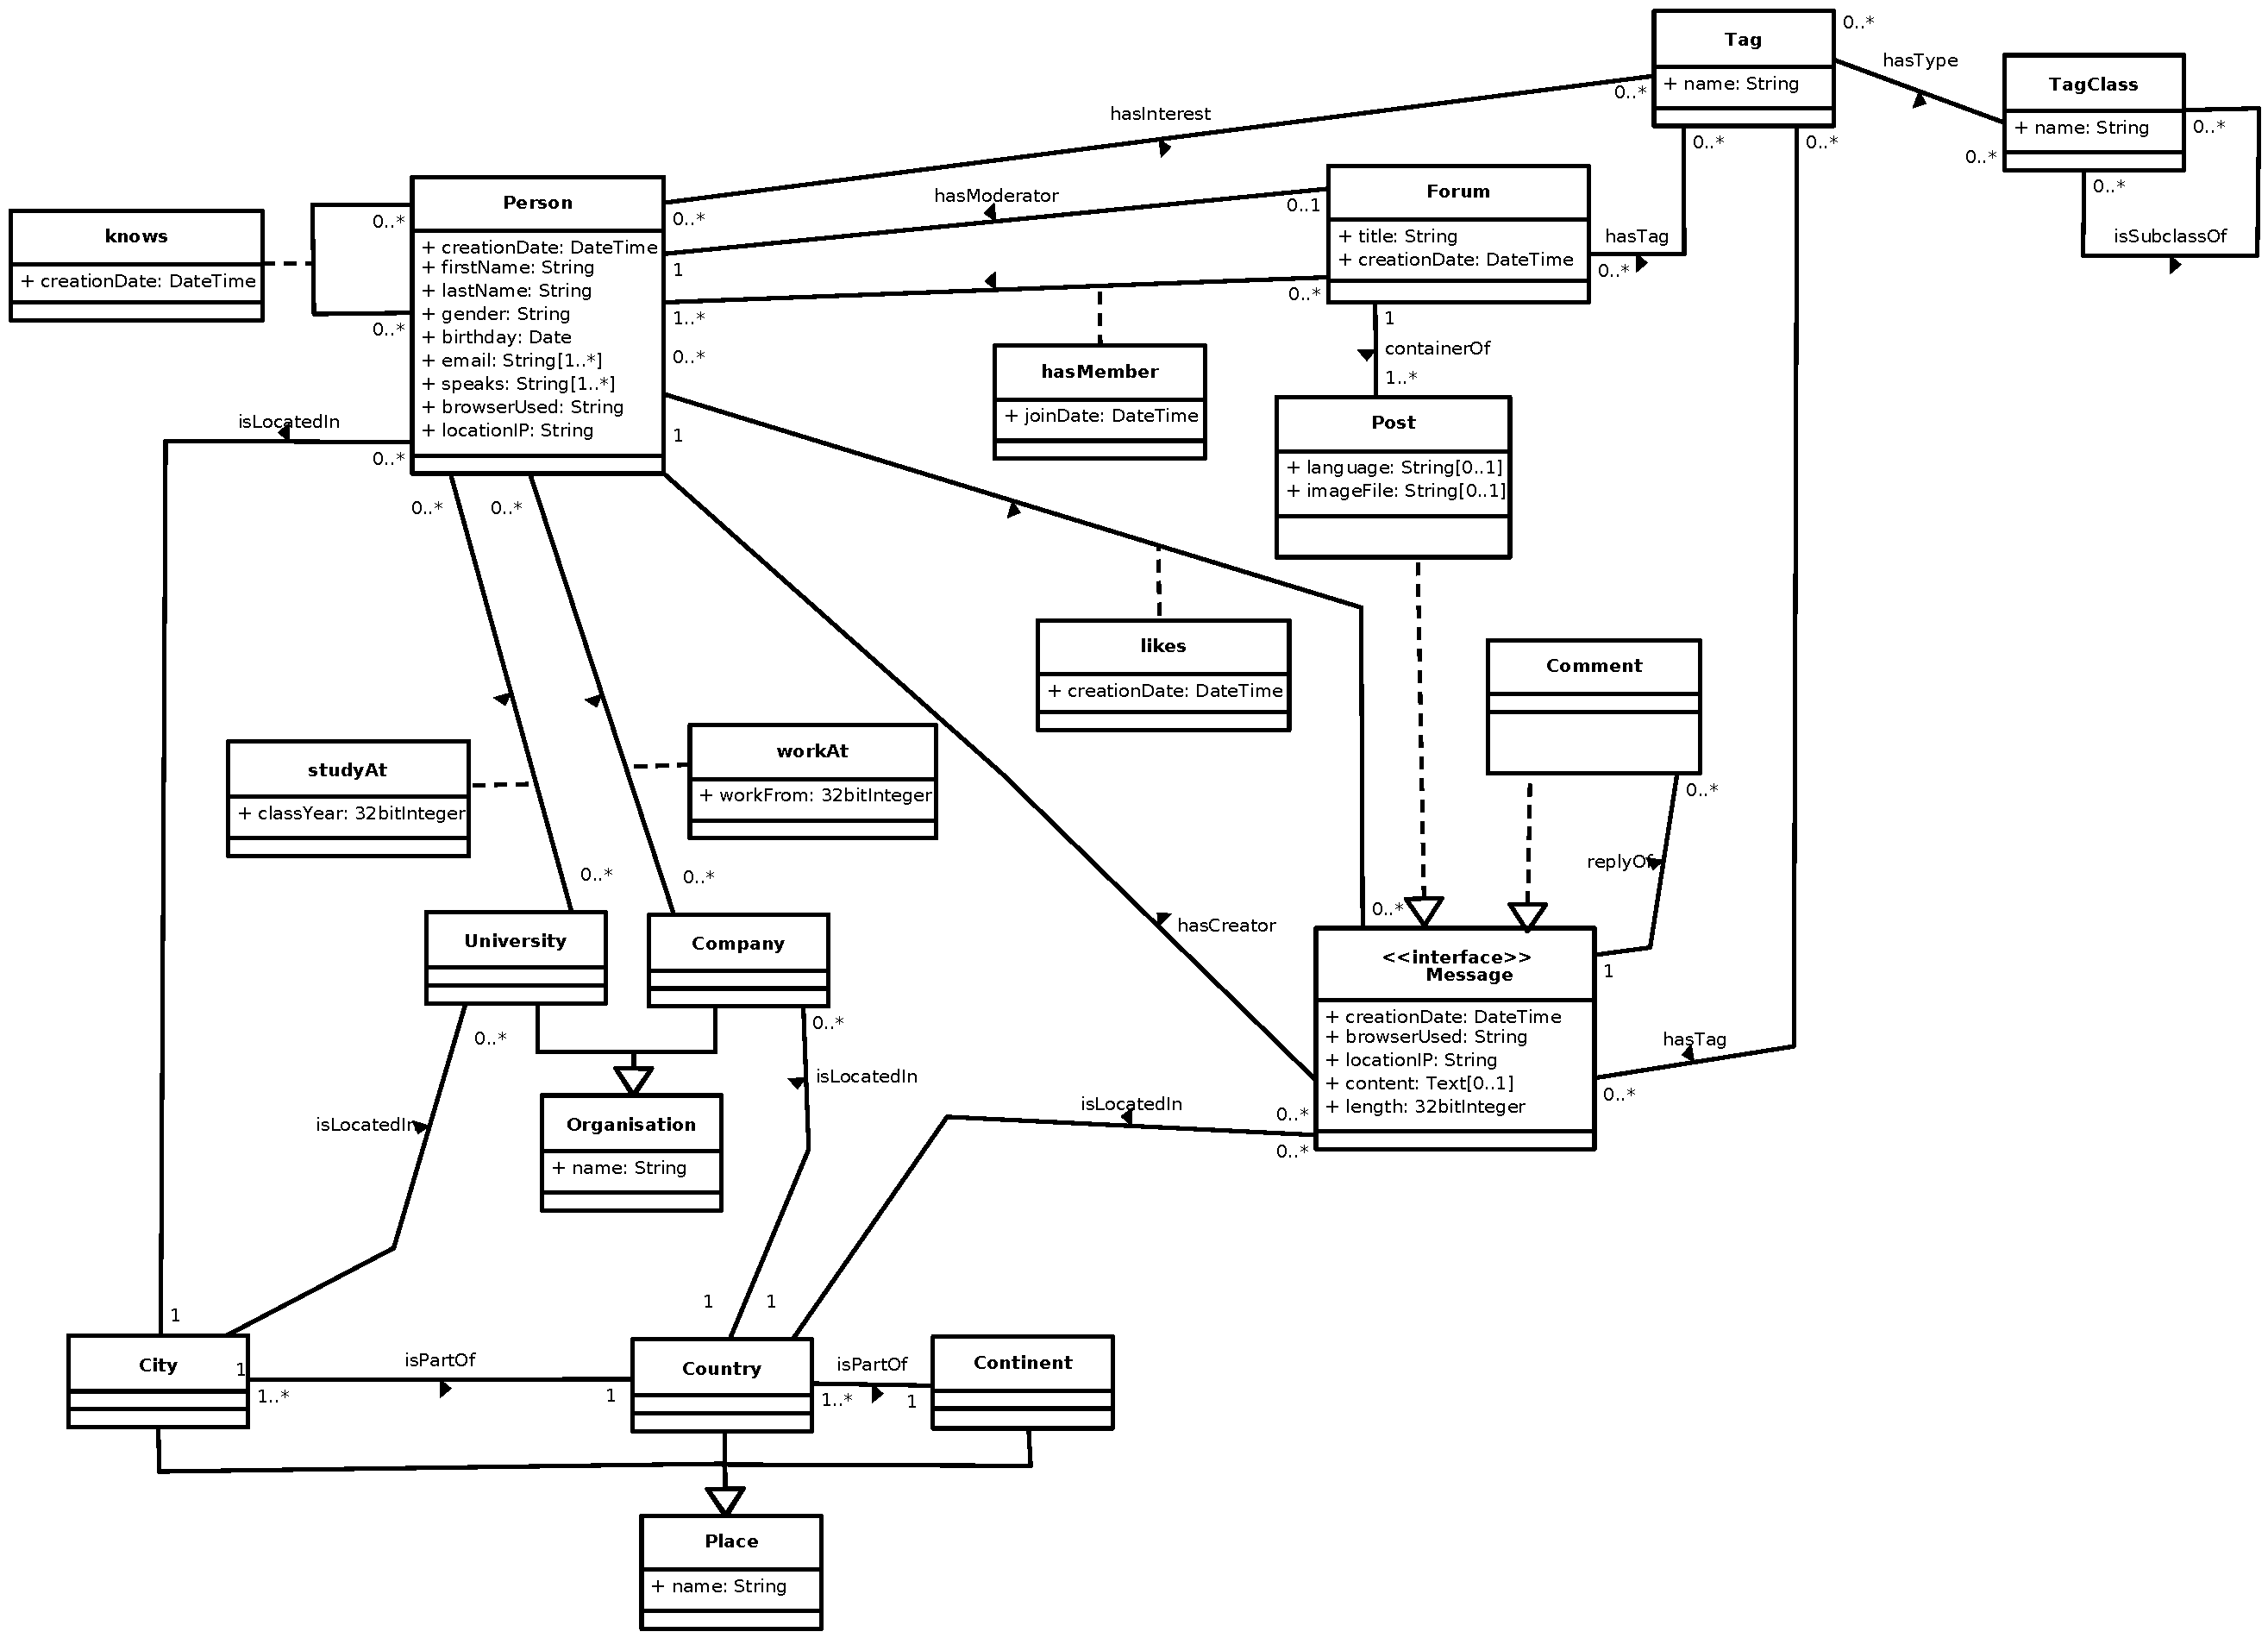
\includegraphics[width=0.9\linewidth]{figures/schema/schema.pdf}
%        \caption{The LDBC-SNB data schema}
%        \label{figure:schema}
%    \end{figure}
%\end{landscape}

\begin{figure}[p]
	\centering
	\rotatebox{90}{
		\begin{minipage}{\textheight}
			\centering
	        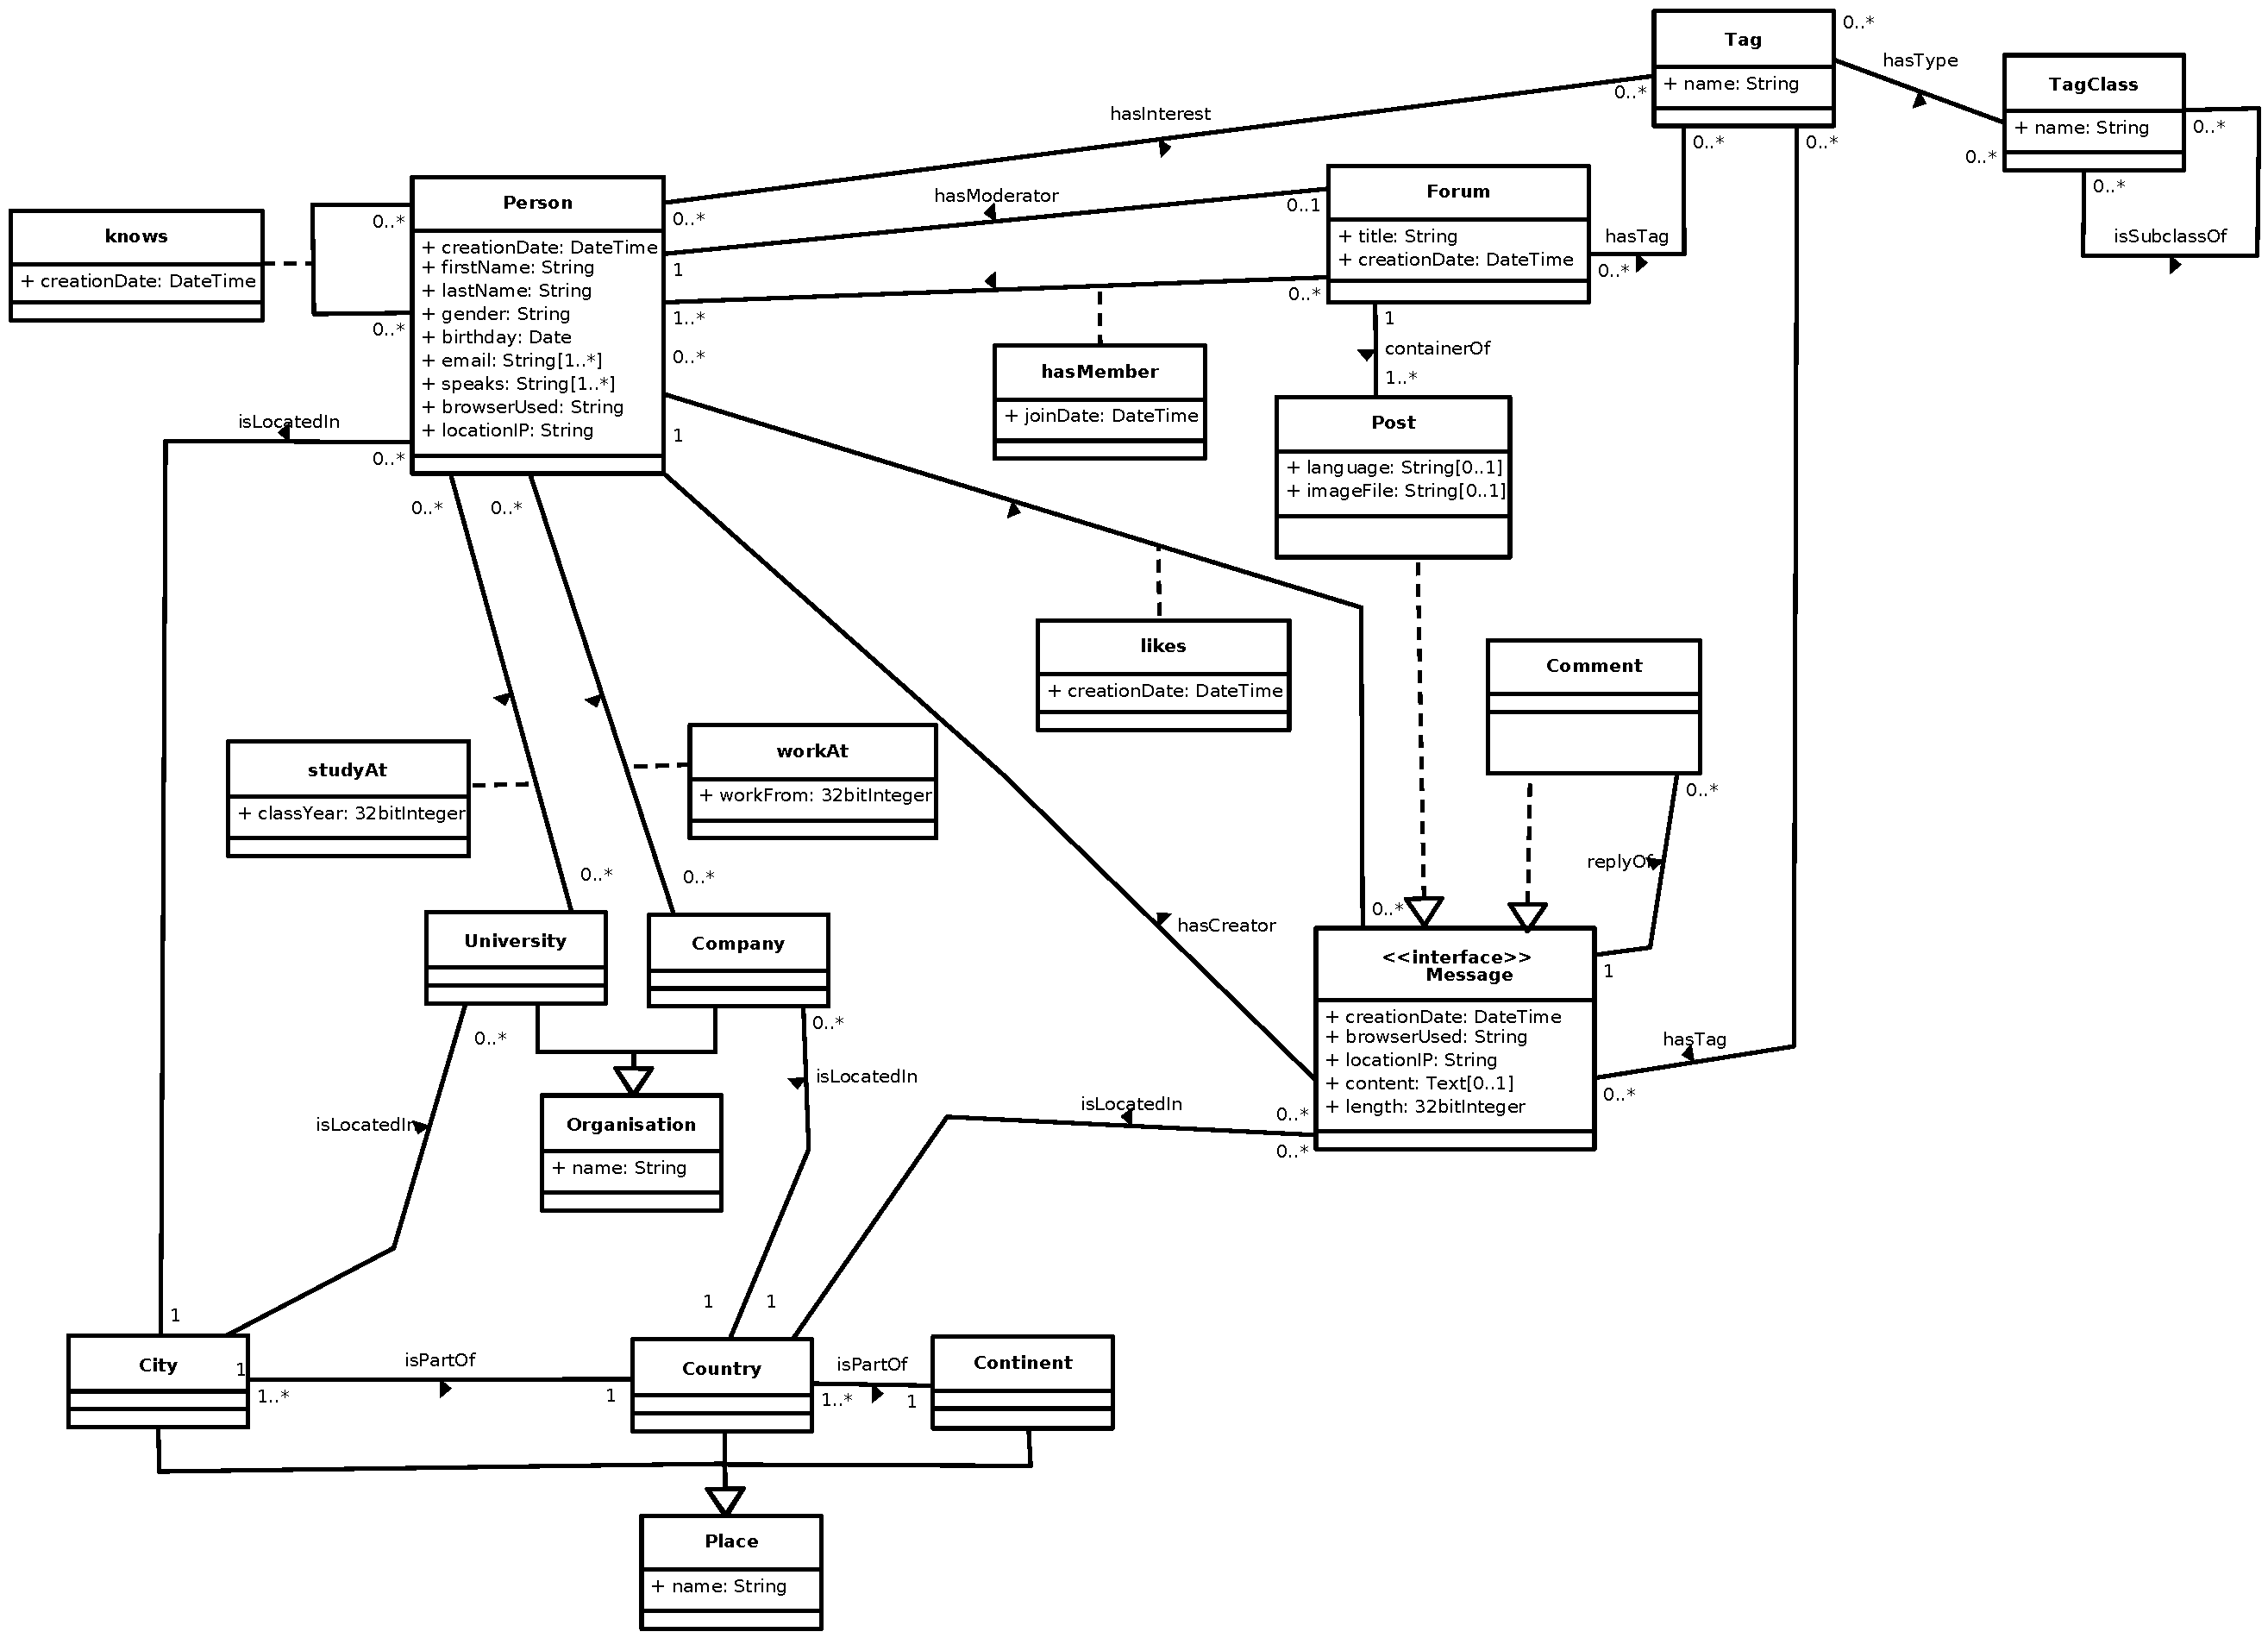
\includegraphics[width=0.9\linewidth]{figures/schema/schema.pdf}
    	    \caption{The LDBC-SNB data schema}
        	\label{figure:schema}
		\end{minipage}
	}
\end{figure}

The schema specifies different entities, their attributes and their relations.
All of them are described in the following sections.

\flushleft{\textbf{Textual Restrictions and Notes}}
\begin{itemize}
    \item Posts have content or imageFile. They have one of them but not both. The one they do not have is an empty string.
    \item Posts in a forum can be created by a non-member person if and only if that person is a modeartor.
\end{itemize}

\subsubsection{Entities}

{\flushleft \textbf{City:}} a sub-class of a Place, and represents a
city of the real world. City entities are used to specify where persons live,
as well as where universities operate.

{\flushleft \textbf{Comment:}} a sub-class of a Message, and represents a
comment made by a person to an existing message (either a Post or a Comment).

{\flushleft \textbf{Company:}} a sub-class of an Organization, and represents a company where persons work.


{\flushleft \textbf{Country:}} a sub-class of a Place, and represents a continent of the real world.


{\flushleft \textbf{Forum:}} a meeting point where people
post messages. Forums are characterized by the topics (represented as tags)
people in the forum are talking about. Although from the schema's perspective
it is not evident, there exist three different types of
forums: persons' personal walls, image albums, and groups. They are
distinguished by their titles. Table~\ref{table:forum} shows the attributes
of Forum entity.

\begin{table}[H]
    \begin{tabular}{|p{2.5cm}|p{2.5cm}|p{10.5cm}|}
        \hline
        \textbf{Attribute} & \textbf{Type} & \textbf{Description} \\
        \hline
        id & ID  & The identifier of the forum.\\
        \hline
        title & Long String  & The title of the forum.\\
        \hline
        creationDate & DateTime  & The date the forum was created\\
        \hline
    \end{tabular}
    \caption{Attributes of Forum entity.}
    \label{table:forum}
\end{table}

{\flushleft \textbf{Message:}} an abstract entity that represents a message
created by a person. Table~\ref{table:message} shows the attributes of Message
abstract entity.

\begin{table}[H]
    \begin{tabular}{|p{2.5cm}|p{2.5cm}|p{10.5cm}|}
        \hline
        \textbf{Attribute} & \textbf{Type} & \textbf{Description} \\
        \hline
        id & ID  & The identifier of the message.\\
        \hline
        browserUsed & String  & The browser used by the Person to create the message.\\
        \hline
        creationDate & DateTime  & The date the message was created.\\
        \hline
        locationIP & String  & The IP of the location from which the message was created.\\
        \hline
        content & Text[0..1]  & The content of the message.\\
        \hline
        length & 32-bit Integer  & The length of the content.\\
        \hline
    \end{tabular}
    \caption{Attributes of Message interface.}
    \label{table:message}
\end{table}

{\flushleft \textbf{Organization:}} an institution of the real
world. Table~\ref{table:organization} shows the attributes of Organization
entity.

\begin{table}[H]
    \begin{tabular}{|p{2.5cm}|p{2.5cm}|p{10.5cm}|}
        \hline
        \textbf{Attribute} & \textbf{Type} & \textbf{Description} \\
        \hline
        id & ID  & The identifier of the organization.\\
        \hline
        name & Long String  & The name of the organization.\\
        \hline
    \end{tabular}
    \caption{Attributes of Organization entity.}
    \label{table:organization}
\end{table}

{\flushleft \textbf{Person:}} the avatar a real world person creates
when he/she joins the network, and contains various information about the
person as well as network related information. Table~\ref{table:person} shows
the attributes of Person entity.

\begin{table}[H]
    \begin{tabular}{|p{2.5cm}|p{2.5cm}|p{10.5cm}|}
        \hline
        \textbf{Attribute} & \textbf{Type} & \textbf{Description} \\
        \hline
        id & ID  & The identifier of the person.\\
        \hline
        firstName & String  & The first name of the person.\\
        \hline
        lastName & String  & The last name of the person.\\
        \hline
        gender & String  & The gender of the person.\\
        \hline
        birthDay & Date  & The birthday of the person .\\
        \hline
        email & Long String[1..*]  & The set of emails the person has.\\
        \hline
        speaks & String[1..*]  & The set of languages the person speaks.\\
        \hline
        browserUser & String  & The browser used by the person when he/she registered to the social network.\\
        \hline
        locationIp & String  & The IP of the location from which the person was registered to the social network.\\
        \hline
        creationDate & DateTime  & The date the person joined the social network.\\
        \hline
    \end{tabular}
    \caption{Attributes of Person entity.}
    \label{table:person}
\end{table}


{\flushleft \textbf{Place:}} a place in the world.
Table~\ref{table:place} shows the attributes of Place entity.

\begin{table}[H]
    \begin{tabular}{|p{2.5cm}|p{2.5cm}|p{10.5cm}|}
        \hline
        \textbf{Attribute} & \textbf{Type} & \textbf{Description} \\
        \hline
        id & ID  & The identifier of the place.\\
        \hline
        name & Long String  & The name of the place.\\
        \hline
    \end{tabular}
    \caption{Attributes of Place entity.}
    \label{table:place}
\end{table}

{\flushleft \textbf{Post:}} a sub-class of Message, that is posted in a
forum. Posts are created by persons into the forums where they belong.
Posts contain either content or imageFile, always one of them but never both.
The one they do not have is an empty string.
Table~\ref{table:post} shows the attributes of Post entity.

\begin{table}[H]
    \begin{tabular}{|p{2.5cm}|p{2.5cm}|p{10.5cm}|}
        \hline
        \textbf{Attribute} & \textbf{Type} & \textbf{Description} \\
        \hline
        language & String[0..1]  & The language of the post.\\
        \hline
        imageFile & String[0..1]  & The image file of the post..\\
        \hline
    \end{tabular}
    \caption{Attributes of Post entity.}
    \label{table:post}
\end{table}

{\flushleft \textbf{Tag:}} a topic or a concept. Tags are used to
specify the topics of forums and posts, as well as the topics a person is
interested in. Table~\ref{table:tag} shows the attributes of Tag entity.

\begin{table}[H]
    \begin{tabular}{|p{2.5cm}|p{2.5cm}|p{10.5cm}|}
        \hline
        \textbf{Attribute} & \textbf{Type} & \textbf{Description} \\
        \hline
        id & ID  & The identifier of the tag.\\
        \hline
        name & Long String  &  The name of the tag.\\
        \hline
    \end{tabular}
    \caption{Attributes of Tag entity.}
    \label{table:tag}
\end{table}

{\flushleft \textbf{TagClass:}} a class or a category used to build
a hierarchy of tags. Table~\ref{table:tagclass} shows the attributes of TagClass
entity.

\begin{table}[H]
    \begin{tabular}{|p{2.5cm}|p{2.5cm}|p{10.5cm}|}
        \hline
        \textbf{Attribute} & \textbf{Type} & \textbf{Description} \\
        \hline
        id & ID  & The identifier of the tagclass.\\
        \hline
        name & Long String  &  The name of the tagclass.\\
        \hline
    \end{tabular}
    \caption{Attributes of TagClass entity.}
    \label{table:tagclass}
\end{table}

{\flushleft \textbf{University:}} a sub-class of Organization,
and represents an institution where persons study.

\subsubsection{Relations}

Relations connect entities of different types. Entities are defined by their ''id'' attribute.

\begin{longtable}{|p{2cm}|p{2.5cm}|p{2.5cm}|p{1cm}|p{7cm}|}
       \hline
        \textbf{Name} & \textbf{Tail} & \textbf{Head} & \textbf{Type} & \textbf{Description} \\
        \hline
        containerOf & Forum[1] & Post[1..*] & D & A Forum and a Post contained in it\\
        \hline
        hasCreator & Message[0..*] & Person[1] & D & A Message and its creator (Person)\\
        \hline
        hasInterest & Person[0..*] & Tag[0..*] & D & A Person and a Tag representing a topic the person is interested in\\
        \hline
        hasMember & Forum[0..*] &  Person[1..*] & D & A  Forum and a member (Person) of the forum
        \begin{itemize}
            \item \textbf{Attribute}: joinDate
            \item \textbf{Type:} DateTime
            \item \textbf{Description:} The Date the person joined the forum
        \end{itemize}
        \\
        \hline
        hasModerator & Forum[0..*] & Person[1] & D & A Forum and its moderator (Person) \\
        \hline
        hasTag & Message[0..*] & Tag[0..*] & D & A Message and a Tag representing the message's topic \\
        \hline
        hasTag & Forum[0..*] & Tag[0..*] & D & A Forum and a Tag representing the forum's topic \\
        \hline
        hasType & Tag[0..*] & TagClass[0..*] & D & A Tag and a TagClass the tag belongs to \\
        \hline
        isLocatedIn & Company[0..*] & Country[1] & D & A Company and its home Country \\
        \hline
        isLocatedIn & Message[0..*] & Country[1] & D & A Message and the Country from which it was issued \\
        \hline
        isLocatedIn & Person[0..*] & City[1] & D & A Person and their home City \\
        \hline
        isLocatedIn & University[0..*] & City[1] & D &  A University and the City where the university is \\
        \hline
        isPartOf & City[1..*] & Country[1] & D & A City and the Country it is part of \\
        \hline
        isPartOf & Country[1..*] & Continent[1] & D & A Country and the Continent it is part of \\
        \hline
        isSubclassOf & TagClass[0..*] & TagClass[0..*] & D & A TagClass its parent TagClass \\
        \hline
        knows & Person[0..*] & Person[0..*] & U & Two Persons that know each other
        \begin{itemize}
            \item \textbf{Attribute}: creationDate
            \item \textbf{Type:} DateTime
            \item \textbf{Description:}  The date the knows relation was established
        \end{itemize}
        \\
        \hline
        likes & Person[0..*] & Message[0..*] & D & A Person that likes a Message
        \begin{itemize}
            \item \textbf{Attribute}: creationDate
            \item \textbf{Type:} DateTime
            \item \textbf{Description:}  The date the like was issued
        \end{itemize}
        \\
        \hline
        replyOf & Comment[0..*] & Message[1] & D & A Comment and the Message it replies \\
        \hline
        studyAt & Person[0..*] & University[0..*] & D & A Person and a University it has studied
        \begin{itemize}
            \item \textbf{Attribute}: classYear
            \item \textbf{Type:} 32-bit Integer
            \item \textbf{Description:} The year the person graduated.
        \end{itemize}
        \\
        \hline
        workAt & Person[0..*] & Company[0..*] & D & A Person and a Company it works
        \begin{itemize}
            \item \textbf{Attribute:} workFrom
            \item \textbf{Type:} 32-bit Integer
            \item \textbf{Description:} The year the person started to work at that company
        \end{itemize}
        \\
        \hline
        \caption{Description of the data relations.}
        \label{table:relations}
\end{longtable}

%\subsection{Data Generation}\label{section:data_generation}
%
%LDBC-SNB provides DATAGEN (Data Base Generator), which produces synthetic
%datasets following the schema described above. Data
%produced mimics a social network's activity during a period of time. Three
%parameters determine the generated data: the number of persons, the number of
%years simulated, and the starting year of simulation. DATAGEN is defined by the
%following characteristics:
%
%\begin{itemize}
%    \item \textbf{Realism.} Data generated by DATAGEN mimics the
%        characteristics of those found in a real social network. In DATAGEN,
%        output attributes, cardinalities, correlations and distributions have
%        been finely tuned to reproduce a real social network in each of its
%        aspects On the one hand, it is aware of the  data and link distributions
%        found in a real social network such as Facebook. On the other hand, it
%        uses real data from DBPedia, such as property dictionaries, which are
%        used to ensure that attribute values are realistic and correlated.
%    \item \textbf{Scalability.} Since LDBC-SNB targets systems of different
%        scales and budgets, DATAGEN is capable of generating datasets of
%        different sizes, from a few Gigabytes to Terabytes. DATAGEN is
%        implemented following the MapReduce parallel paradigm, allowing the
%        generation of small datasets in single node machines, as well as large
%        datasets on commodity clusters.
%    \item \textbf{Determinism.} DATAGEN is deterministic regardless of the number
%        of cores/machines used to produce the data. This important feature
%        guarantees that all Test Sponsors will face the same dataset,
%        thus, making the comparisons between different systems fair and the
%        benchmarks' results reproducible.
%    \item \textbf{Usability.} LDBC-SNB is designed to have an affordable entry
%        point. As such, DATAGEN's design is  severely influenced by this
%        philosophy, and therefore it is designed to be as easy to use as
%        possible.
%\end{itemize}
%
%
%\subsubsection{Resource Files}
%
%DATAGEN uses a set of resource files with data
%extracted from DBpedia. Conceptually, DATAGEN generates attribute's
%values following a property dictionary model that is defined by
%
%\begin{itemize}
%    \item a dictionary $D$
%    \item a ranking function $R$
%    \item a probability function $F$
%\end{itemize}
%
%Dictionary D is a fixed set of values. The ranking function R is a bijection
%that assigns to each value in a dictionary a unique rank between 1 and |$D$|.
%The probability density function $F$ specifies how the data generator chooses
%values from dictionary $D$ using the rank for each term in the dictionary. The
%idea to have a separate ranking and probability function is motivated by the
%need of generating correlated values: in particular, the ranking function is
%typically parameterized by some parameters: different parameter values result
%in different rankings. For example, in the case of a dictionary of property
%firstName, the popularity of first names, might depend on the gender, country
%and birthDate properties. Thus, the fact that the popularity of first names in
%different countries and times is different, is reflected by the different ranks
%produced by function $R$ over the full dictionary of names.  DATAGEN uses a
%dictionary for each literal property, as well as ranking functions for all
%literal properties. These are materialized in a set of resource files, which
%are described in Table~\ref{table:property_dictionaries}.
%
%\begin{table}[H]
%\begin{tabular}{|p{4cm}|p{12cm}|}
%    \hline
%    \textbf{Resource Name} & \textbf{Description} \\
%    \hline
%    Browsers & Contains a list of web browsers and their probability to be used. It is used to set the browsers used by the users.\\
%    \hline
%    Cities by Country & Contains a list of cites and the country they belong. It is used to assign cities to users and universities.\\
%    \hline
%    Companies by Country & Contains the set of companies per country. It is used to set the countries where companies operate.\\
%    \hline
%    Countries & Contains a list of countries and their populations. It is used to obtain the amount of people generated for each country.\\
%    \hline
%    Emails & Contains the set of email providers. It is used to generate the email accounts of persons.\\
%    \hline
%    IP Zones & Contains the set of IP ranges assigned to each country. It is used to assign the IP addresses to users.\\
%    \hline
%    Languages by Country & Contains the set of languages spoken in each country. It is used to set the languages spoken by each user.\\
%    \hline
%    Name by Country & Contains the set of names and the probability to appear in each country. It is used to assign names to persons, correlated with their countries.\\
%    \hline
%    Popular places by Country & Contains the set of popular places per country. These are used to set where images attached to posts are taken from.\\
%    \hline
%    Surnames' by Country & Contains the set of surnames and the probability to appear in each country. It is used to assign surnames to persons, correlated with their countries.\\
%    \hline
%    Tags by Country & Contains a set of tags and their probability to appear in each country. It is used to assign the interests to persons and forums.\\
%    \hline
%    Tag Classes & Contains, for each tag, the classes it belongs to.\\
%    \hline
%    Tag Hierarchies & Contains, for each tagClass, their parent tagClass.\\
%    \hline
%    Tag Matrix & Contains, for each tag, the correlation probability with the other tags. It is used enrich the tags associated to messages.\\
%    \hline
%    Tag Text & Contains, for each tag, a text. This is used to generate the text for messages.\\
%    \hline
%    Universities by City & Contains the set of universities per city. It is used to set the cities where universities operate.\\
%    \hline
%\end{tabular}
%    \caption{Resource files}
%    \label{table:property_dictionaries}
%\end{table}
%
%\subsubsection{Graph Generation}
%
%Figure~\ref{figure:generation_process} conceptually depicts the full data
%generation process. The first step loads all the dictionaries and resource
%files, and initializes the DATAGEN parameters.  Second, it generates all the
%Persons in the graph, and the minimum necessary information to operate. Part of
%these information are the interests of the persons, and the number of knows
%relationships of every person, which is guided by a degree distribution
%function similar to that found in Facebook~\cite{facebook_anatomy}.
%
%The next three steps are devoted to the creation of knows relationships.  An
%important aspect of real social networks, is the fact that similar persons
%(with similar interests and behaviors) tend to be connected. This is known as
%the Homophily principle~\cite{mcpherson2001birds}, and implies the presence of
%a larger amount of triangles than that expected in a random network. In order
%to reproduce this characteristic, DATAGEN generates the edges by means of
%correlation dimensions.  Given a person, the probability to be connected to
%another person is typically skewed with respect to some similarity between the
%persons. That is, for a person $n$ and for a small set of persons that are
%somehow similar to it, there is a high connectivity probability, whereas for
%most other persons, this probability is quite low. This knowledge is
%exploited by DATAGEN to reproduce correlations.
%
%\begin{figure}[H]
%    \centering
%    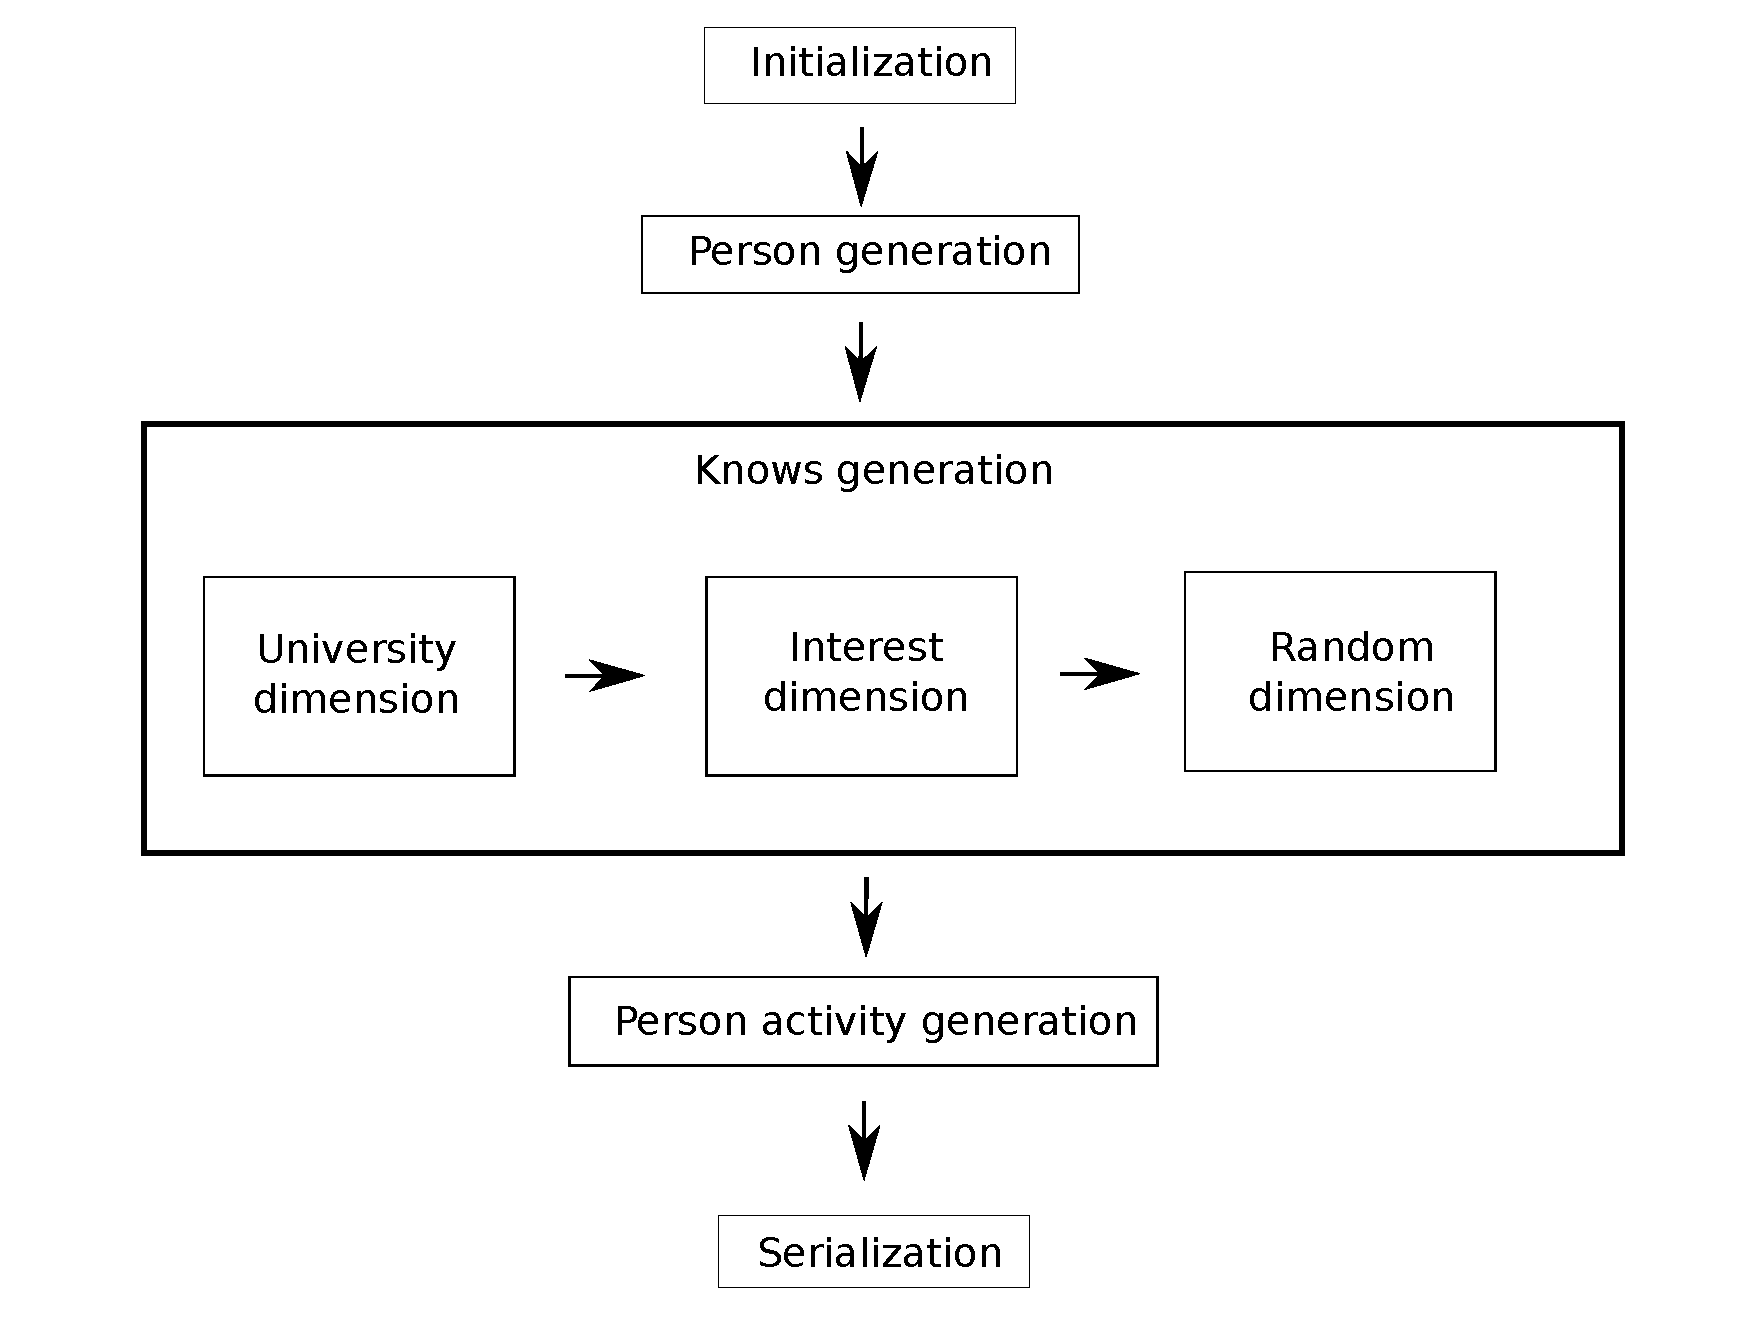
\includegraphics[width=1\linewidth]{figures/sndg/execution.pdf}
%    \caption{The DATAGEN generation process.}
%    \label{figure:generation_process}
%\end{figure}
%
%Given a similarity function $M(x) : n → [0, \infty]$ that gives a score to a person,
%with the characteristic that two similar persons will have similar scores, we
%can sort all the persons by function $M$ and compare a person n against only the
%W neighboring persons in the sorted array. The consequence of this approach is
%that similar persons are grouped together, and the larger the
%distance between two persons indicates a monotonic increase in their similarity
%difference. In order to choose the persons to connect, DATAGEN uses a geometric
%probability distribution that provides a probability for picking persons to
%connect, that are between 1 and $W$ positions apart in the similarity
%ranking.
%
%Similarity functions and probability distribution functions over ranked
%distance drive what kind of persons will be connected with an edge, not how
%many. As stated above, the number of friends of a person is determined by a
%Facebook-like distribution. The edges that will be connected to a person $n$,
%are selected by randomly picking the required number of edges according to the
%correlated probability distributions as discussed before. In the case that
%multiple correlations exist, another probability function is used to divide the
%intended number of edges between the various correlation dimensions. In DATAGEN,
%three correlated dimensions are chosen: the first one depends on where the
%person studied and when, and the second correlation dimension depends on the
%interests of the person, and the third one is random (to reproduce the random
%noise present in real data). Thus, DATAGEN has a Facebook-like distributed node
%degree, and a predictable (but not fixed) average split between the reasons for
%creating edges.
%
%In the next step, person's activity, in the form of forums, posts and comments
%is created. DATAGEN reproduces the fact that people with a larger number of
%friends have a higher activity, and hence post more photos and comments to a
%larger number of posts. Another important characteristic of real users'
%activity in social network, are time correlations.  Usually, users' posts
%creation in a social network is driven by real world events.  For
%instance, one may think about an important event such as the elections in a
%country, or a natural disaster. Around the time these events occur, network
%activity about these events' topics sees an increase in volume. DATAGEN
%reproduces these characteristics with the simulation of what we name as
%flashmob events.  Several events are generated randomly at the beginning of the
%generation process, which are assigned a random tag, and are given a time and
%an intensity which represents the repercussion of the event in the real world.
%When persons' posts are created, some of them are classified as flashmob posts,
%and their topics and dates are assigned based on the generated flashmob events.
%The volume of activity around this events is modeled following a model similar
%to that described in~\cite{flashmobs}. Furthermore, in order to reproduce the
%more uniform every day's user activity, DATAGEN also generates post uniformly
%distributed along all the simulated time.
%
%Finally, in the last step the data is serialized into the output files.
%
%\subsubsection{Implementation Details}
%
%DATAGEN is implemented using the MapReduce parallel paradigm. In MapReduce, a
%Map function runs on different parts of the input data, in parallel and on many
%node clusters. This function processes the input data and produces for each
%result a key. Reduce functions then obtain this data and Reducers run in
%parallel on many cluster nodes. The produced key simply determines the Reducer
%to which the results are sent. The use of the MapReduce paradigm allows the
%generator to scale considerably, allowing the generation of huge datasets by
%using clusters of machines.
%
%In the case of DATAGEN, the overall process is divided into three MapReduce jobs.
%In the first job, each mapper generates a subset of the persons of the graph. A
%key is assigned to each person using one of the similarity functions described
%above. Then, reducers receive the the key-value pairs sorted by the key,
%generate the knows relations following the described windowing process, and
%assign to each person a new key based on another similarity function, for the
%next MapReduce pass.  This process can be successively repeated for additional
%correlation dimension.  Finally, the last reducer generates the remaining
%information such as forums, posts and comments.
%

\subsection{Output Data}

DATAGEN produces outputs three different items:
\begin{itemize}
  \item \textbf{Dataset}: The dataset to be bulk loaded by the SUT. It
    corresponds to roughly the 90\% of the total generated network.
  \item \textbf{Update Streams}: A set of update streams containing update
    queries, which are used by the driver to generate the update queries of the
    workloads. This update
    streams correspond to the remaining 10\% of the generated dataset.
  \item \textbf{Substitution Parameters}: A set of files containing the
    different parameter bindings that will be used by the driver to generate the
    read queries of the workloads.
\end{itemize}

The SUT have to take care only of the generated Dataset to be bulk loaded.
Three different formats are supported by DATAGEN:

\begin{itemize}
  \item \textbf{CSV:} Data output in CSV format, one file per different entity and on file
    per different relation. Also, there is a file por those attributes whose
    cardinality is larger than one (\ie Person.email, Person.speaks, \etc).
  \item \textbf{CSVMergeForeign:} Similar to CSV format, but in this case, those
    relations of the form 1 to 1 and 1 to N, are stored in the tail entity file as
    a foreign keys.
  \item \textbf{Turtle:} Dataset in turtle format for RDF systems.
\end{itemize}



\subsubsection{CSV}

This is a comma separated format. Each entity, relation and properties with a
cardinality larger than one, are output in a separate file. Generated files are
summarized at Table~\ref{table:csv}.  Depending on the number of threads used
for generating the dataset, the number of files varies, since there is a file
generated per thread. The * in the file names indicates a number between 0 and
$\mathit{NumberOfThreads}-1$.

\begin{table}[htbp]
	\centering
	\rotatebox{90}{
	\begin{minipage}[c]{\textheight}
        \footnotesize
        \centering
        \begin{tabular}{|p{5cm}|p{19cm}|}
            \hline
            \textbf{File} & \textbf{Content} \\
            \hline
            comment\_*.csv & id | creationDate | locationIP | browserUsed | content | length |\\
            \hline
            comment\_hasCreator\_person\_*.csv & Comment.id | Person.id |\\
            \hline
            comment\_isLocatedIn\_place\_*.csv & Comment.id | Place.id |\\
            \hline
            comment\_replyOf\_comment\_*.csv & Comment.id | Comment.id |\\
            \hline
            comment\_replyOf\_post\_*.csv &  Comment.id | Post.id |\\
            \hline
            forum\_*.csv & id | title | creationDate |\\
            \hline
            forum\_containerOf\_post\_*.csv & Forum.id | Post.id |\\
            \hline
            forum\_hasMember\_person\_*.csv & Forum.id | Person.id | joinDate |\\
            \hline
            forum\_hasModerator\_person\_*.csv & Forum.id | Person.id |\\
            \hline
            forum\_hasTag\_tag\_*.csv & Forum.id | Tag.id |\\
            \hline
            organization\_*.csv & id | type({"university", "company"}) | name | url |\\
            \hline
            organisation\_isLocatedIn\_place\_*.csv & Organisation.id | Place.id |\\
            \hline
            person\_*.csv & id | firstName | lastName | gender | birthday | creationDate | locationIP | browserUsed |\\
            \hline
            person\_email\_emailaddress\_*.csv & Person.id | email |\\
            \hline
            person\_hasInterest\_tag\_*.csv &  Person.id | Tag.id |\\
            \hline
            person\_isLocatedIn\_place\_*.csv & Person.id | Place.id |\\
            \hline
            person\_knows\_person\_*.csv & Person.id | Person.id | creationDate |\\
            \hline
            person\_likes\_comment\_*.csv & Person.id | Post.id | creationDate |\\
            \hline
            person\_likes\_post\_*.csv & Person.id | Post.id | creationDate |\\
            \hline
            person\_speaks\_language\_*.csv & Person.id | language |\\
            \hline
            person\_studyAt\_organisation\_*.csv & Person.id | Organisation.id | classYear |\\
            \hline
            person\_workAt\_organisation\_*.csv &  Person.id | Organisation.id | workFrom |\\
            \hline
            place\_*.csv & id | name | url | type({"city", "country", "continent"}) |\\
            \hline
            place\_isPartOf\_place\_*.csv & Place.id | Place.id |\\
            \hline
            post\_*.csv & id | imageFile | creationDate | locationIP | browserUsed | language | content | length |\\
            \hline
            post\_hasCreator\_person\_*.csv & Post.id | Person.id |\\
            \hline
            post\_hasTag\_tag\_*.csv & Post.id | Tag.id |\\
            \hline
            post\_isLocatedIn\_place.csv & Post.id | Place.id |\\
            \hline
            tag\_*.csv & id | name | url | \\
            \hline
            tag\_hasType\_tagclass\_*.csv & Tag.id | TagClass.id |\\
            \hline
            tagclass\_*.csv & id | name | url | \\
            \hline
            tagclass\_isSubclassOf\_tagclass\_*.csv & TagClass.id | TagClass.id |\\
            \hline
        \end{tabular}
        \caption{Files output by CSV serializer}
        \label{table:csv}
	\end{minipage}
	}
\end{table}




\subsubsection{CSV\_MERGE\_FOREIGN}

This is a comma separated format. It is similar to CSV, but those relations
connecting two entities A and B, where an entity A has a cardinality of one, A
is output as a column of entity B. Generated files are summarized at
Table~\ref{table:csv_merge_foreign}. Depending on the number of threads used for generating
the dataset, the number of files varies, since there is a file generated per
thread. The * in the file names indicates a number between 0 and $\mathit{NumberOfThreads}-1$.

\begin{table}[htbp]
	\centering
	\rotatebox{90}{
		\begin{minipage}[c]{\textheight}
        \footnotesize
        \centering
        \begin{tabular}{|p{5cm}|p{19cm}|}
            \hline
            \textbf{File} & \textbf{Content} \\
            \hline
            comment\_*.csv & id | creationDate | locationIP | browserUsed | content | length | creator | place | replyOfPost | replyOfComment |\\
            \hline
            forum\_*.csv & id | title | creationDate | moderator |\\
            \hline
            forum\_hasMember\_person\_*.csv & Forum.id | Person.id | joinDate |\\
            \hline
            forum\_hasTag\_tag\_*.csv & Forum.id | Tag.id |\\
            \hline
            organization\_*.csv & id | type({"university", "company"}) | name | url |\\
            \hline
            organisation\_isLocatedIn\_place\_*.csv & Organisation.id | Place.id |\\
            \hline
            person\_*.csv & id | firstName | lastName | gender | birthday | creationDate | locationIP | browserUsed | place |\\
            \hline
            person\_email\_emailaddress\_*.csv & Person.id | email |\\
            \hline
            person\_hasInterest\_tag\_*.csv &  Person.id(Long) | Tag.id |\\
            \hline
            person\_knows\_person\_*.csv & Person.id | Person.id  | creationDate |\\
            \hline
            person\_likes\_comment\_*.csv & Person.id | Post.id | creationDate |\\
            \hline
            person\_likes\_post\_*.csv & Person.id | Post.id | creationDate |\\
            \hline
            person\_speaks\_language\_*.csv & Person.id | language |\\
            \hline
            person\_studyAt\_organisation\_*.csv & Person.id | Organisation.id | classYear |\\
            \hline
            person\_workAt\_organisation\_*.csv &  Person.id | Organisation.id | workFrom |\\
            \hline
            place\_*.csv & id | name | url | type({"city", "country", "continent"}) |\\
            \hline
            place\_isPartOf\_place\_*.csv & Place.id | Place.id |\\
            \hline
            post\_*.csv & id | imageFile | creationDate | locationIP | browserUsed | language | content | length | creator | Forum.id | place |\\
            \hline
            post\_hasTag\_tag\_*.csv & Post.id | Tag.id |\\
            \hline
            tag\_*.csv & id | name | url | \\
            \hline
            tag\_hasType\_tagclass\_*.csv & Tag.id | TagClass.id |\\
            \hline
            tagclass\_*.csv & id | name | url | \\
            \hline
            tagclass\_isSubclassOf\_tagclass\_*.csv & TagClass.id | TagClass.id |\\
            \hline
        \end{tabular}
        \caption{Files output by CSV\_MERGE\_FOREIGN serializer}
        \label{table:csv_merge_foreign}
	\end{minipage}
}
\end{table}


\subsubsection{Turtle}

This is the standard Turtle\footnote{Description of
the Turtle RDF format http://www.w3.org/TR/turtle/} format. DATAGEN outputs
two files: \texttt{0\_ldbc\_socialnet\_static\_dbp.ttl} and \texttt{0\_ldbc\_socialnet.ttl}.

\subsection{Scale Factors}

LDBC-SNB defines a set of scale factors (SFs), targeting systems of different
sizes and budgets.  SFs are computed based on the ASCII size in Gigabytes of
the generated output files using the CSV serializer. For example, SF 1 weights roughly 1~GB in CSV
format, SF 3 weights roughly 3~GB and so on and so forth.  The proposed SFs are
the following: 1, 3, 10, 30, 100, 300, 1000. The Test Sponsor may select the SF
that better fits their needs, by properly configuring the DATAGEN.
% , as described in Section~\ref{section:data_generation}.

The size of the resulting dataset, is mainly affected by the following
configuration parameters: the number of persons and the number of years
simulated. Different SFs are computed by scaling the number of Persons in
the network, while fixing the number of years simulated.
Table~\ref{tab:snsize} shows the parameters used in each of the SFs.

\begin{table}[H]
\centering
\begin{tabular}{|c||r|r|r|r|r|r|r|}
\hline  Scale Factor  & 1 &  3 & 10 & 30 & 100 & 300 & 1000 \\
\hline  \# of Persons  & 11K &  27K & 73K & 182K & 499K & 1.25M & 3.6M \\
\hline  \# of Years  & 3 &  3 & 3 & 3 & 3 & 3 & 3 \\
\hline  Start Year & 2010 &  2010 & 2010 & 2010 & 2010 & 2010 & 2010 \\
\hline
\end{tabular}
\centering
\caption{Parameters of each scale factor.}
\label{tab:snsize}
\end{table}

For example, SF 30 consists of the activity of a social network of 182K users
during a period of three years, starting from 2010.

%In
%Appendix~\ref{appendix:scale_factors}, we show the statistics of each of the
%proposed SFs in detail, including distributions for some of the relations.

%%%%%%%%%%%%%%%%%%%%%%%%%%%%%%%%%%%%%%%%%%%%%%%%%%%%%%%%%%%%%%%%%%%%%%%%%%%%%%
%%%%%%%%%%%%%%%%%%%%%%%%%%%%%%%%%%%%%%%%%%%%%%%%%%%%%%%%%%%%%%%%%%%%%%%%%%%%%%
%%%%%%%%%%%%%%%%%%%%%%%%%%%%%%%%%%%%%%%%%%%%%%%%%%%%%%%%%%%%%%%%%%%%%%%%%%%%%%

\chapter{Workloads}
\label{section:workloads}

%%%%%%%%%%%%%%%%%%%%%%%%%%%%%%%%%%%%%%%%%%%%%%%%%%%%%%%%%%%%%%%%%%%%%%%%%%%%%%
%%%%%%%%%%%%%%%%%%%%%%%%%%%%%%%%%%%%%%%%%%%%%%%%%%%%%%%%%%%%%%%%%%%%%%%%%%%%%%
%%%%%%%%%%%%%%%%%%%%%%%%%%%%%%%%%%%%%%%%%%%%%%%%%%%%%%%%%%%%%%%%%%%%%%%%%%%%%%

\section{Query Description Format}
\label{sub:queries_structure}
Queries are described in natural language using a well-defined structure that consists of three sections:
\textit{description}, a concise textual description of the query;
\textit{parameters}, a list of input parameters and their types;
and \textit{results}, a list of expected results and their types.
The syntax used in \textit{parameters} and \textit{results} sections is as follows:

\begin{itemize}
    \item \textbf{Entity}: entity type in the dataset.\\
        One word, possibly constructed by appending multiple words together, starting with uppercase character and following the camel case notation,
        \eg \texttt{TagClass} represents an entity of type ``TagClass''.
    \item \textbf{Relationship}: relationship type in the dataset.\\
        One word, possibly constructed by appending multiple words together, starting with lowercase character and following the camel case notation,
        and surrounded by arrow to communicate direction,
        \eg \mbox{\texttt{-worksAt->}} represents a directed relationship of type ``worksAt''.
    \item \textbf{Attribute}: attribute of an entity or relationship in the dataset.\\
        One word, possibly constructed by appending multiple words together, starting with lowercase character and following the camel case notation,
        and prefixed by a ``.'' to dereference the entity/relationship,
        \eg \texttt{Person.firstName} refers to ``firstName'' attribute on the ``Person'' entity,
        and \mbox{\texttt{-studyAt->.classYear}} refers to ``classYear'' attribute on the ``studyAt'' relationship.
    \item \textbf{Unordered Set}: an unordered collection of distinct elements.\\
        Surrounded by \{ and \} braces, with the element type between them,
        \eg \texttt{\{String\}} refers to a set of strings.
    \item \textbf{Ordered List}: an ordered collection where duplicate elements are allowed.\\
        Surrounded by [ and ] braces, with the element type between them,
        \eg \texttt{[String]} refers to a list of strings.
    \item \textbf{Ordered Tuple}: a fixed length, fixed order list of elements, where elements at each position of the tuple have predefined, possibly different, types. \\
        Surrounded by < and > braces, with the element types between them in a specific order
        \eg \texttt{<String, Boolean>} refers to a 2-tuple containing a string value in the first element and a boolean value in the second,
        and \texttt{[<String, Boolean>]} is an ordered list of those 2-tuples.
\end{itemize}

\paragraph{Categorization of results.} Results are categorized according to their source of origin:

\begin{itemize}
	\item \textbf{Raw} (\texttt{R}), if the result is returned with an unmodified value and type.
	\item \textbf{Calculated} (\texttt{C}), if the result is calculated from other values and conditions.
	\item \textbf{Aggregated} (\texttt{A}), if the result is an aggregated value, \eg a count or a sum of another value. If a result is both calculated and aggregated (\eg $\mathsf{count(x) + count(y)}$ or $\mathsf{avg(x + y)}$), it is considered an aggregated result.
	\item \textbf{Meta} (\texttt{M}), if the result is based on type information, \eg the type of the node.
\end{itemize}


%%%%%%%%%%%%%%%%%%%%%%%%%%%%%%%%%%%%%%%%%%%%%%%%%%%%%%%%%%%%%%%%%%%%%%%%%%%%%%
%%%%%%%%%%%%%%%%%%%%%%%%%%%%%%%%%%%%%%%%%%%%%%%%%%%%%%%%%%%%%%%%%%%%%%%%%%%%%%
%%%%%%%%%%%%%%%%%%%%%%%%%%%%%%%%%%%%%%%%%%%%%%%%%%%%%%%%%%%%%%%%%%%%%%%%%%%%%%

\section{Conventions for Query Definitions}

\paragraph{Interval notations.} Closed interval boundaries are denoted with 
\texttt{[} 
and \texttt{]}, while open interval boundaries are denoted with \texttt{(} and 
\texttt{)}. For example, \texttt{[0, 1)} denoted an interval between 0 and 1, 
closed on the left and open on the right.

\paragraph{Comparing Date and DateTime values.}

Some query specifications (\eg \queryRefCard{bi-read-01}{BI}{1}, 
\queryRefCard{bi-read-02}{BI}{2}, etc.) require implementations to compare a 
$\mathsf{DateTime}$ value with a $\mathsf{Date}$ value. In these cases, the 
$\mathsf{Date}$ value should be implicitly converted $\mathsf{DateTime}$ value 
with a time of 00:00:00.000+0000 (\ie with the timezone of GMT).

\paragraph{Matching semantics.}

Unless noted otherwise, the specification uses \emph{homomorphic} matching 
semantics~\cite{Angles:2017:FMQ:3145473.3104031}, \ie both nodes and edges can 
occur multiple times in a match. Note that for variable length path, duplicate 
edges are not allowed.

\paragraph{Aggregation semantics.}

The \lstinline{count} aggregation always requires the query to determine the number of \emph{distinct} elements (nodes or edges). For example, this can be achieved in the Cypher, SPARQL and SQL query languages with the \lstinline[language=sql]{count(DISTINCT ...)} construct.

\paragraph{Graph patterns.}

To illustrate queries, we use graph patterns such as \autoref{fig:example-graph-pattern} with the following notation:

\begin{figure}[ht]
	\begin{center}
		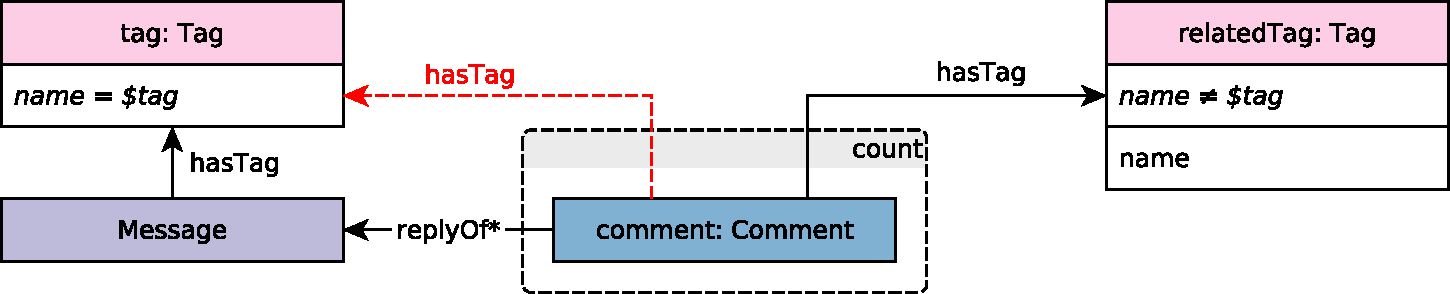
\includegraphics[scale=\patternscale,margin=0cm .2cm]{patterns/bi-read-08}
		\caption{Example graph pattern.}
		\label{fig:example-graph-pattern}
	\end{center}
\end{figure}

\begin{itemize}
	\item Nodes are marked as $\mathsf{entityName: EntityType}$ (camel case 
	notation for both, starting with a lowercase character for the first and an 
	uppercase character for the second). If the $\mathsf{entityName}$ is not used 
	in the query results, aggregations or calculations, and not referenced in the 
	query specification, the $\mathsf{entityName}$ can be omitted.
	\item Positive conditions for edges are denoted with solid lines.
	\item Negative conditions for edges, \ie edges that are not allowed in the graph, are denoted with \textcolor{red}{\dashuline{dashed red}} lines.
	\item Edges without direction imply that there must be an edge in \emph{at least one of the directions}.
	\item Filtering conditions are typeset in \textit{italic}, \eg $\mathit{id} = 
	\mathit{\textdollar tag}$.
	\item Attributes that should be returned are denoted in sans-serif font, \eg $\mathsf{name}$.
	\item Variable length paths, \ie edges that can be traversed multiple times 
	are denoted with $*\mathsf{min}...\mathsf{max}$, \eg $\mathsf{replyOf}*$ or 
	$\mathsf{knows*1 \ldots 2}$. By default, the value of $\mathsf{min}$ is 1, 
	and the value of $\mathsf{max}$ is unlimited.
	\item Aggregations are shown in dashed boxes with the type of aggregation ($\mathsf{count}$, $\mathsf{sum}$, $\mathsf{avg}$, etc.) in the upper right corner.
\end{itemize}

\newcommand{\tuple}[1]{\langle #1 \rangle}

\paragraph{Keywords.} The pattern notation uses a small set of keywords:

\begin{itemize}
	\item $\mathsf{UNWIND}$ unnests a list, \ie produces a set of one-tuples. For 
	example, $\mathsf{UNWIND} [1, 2, 3]$ results in $ \{ \tuple{1}, \tuple{2}, 
	\tuple{3} \} $.
	\item Aggregation operations: \lstinline{count}, \lstinline{avg}. % \lstinline{sum} - sum is not used in the figures as we always sum some derived value
	\item Functions:
	\begin{itemize}
		\item \lstinline{floor(x)} (returns $\lfloor x \rfloor$),
		\item \lstinline{year(date)} (extracts the year from a given date),
		\item \lstinline{month(date)} (extracts the month from a given date).
	\end{itemize}
\end{itemize}

\paragraph{Resolving ambiguity.} Note that if the textual description and the graph pattern are different for a particular query (either due to an error or the lack of sophistication in the graphical syntax), \emph{the textual description takes precedence}.

%%%%%%%%%%%%%%%%%%%%%%%%%%%%%%%%%%%%%%%%%%%%%%%%%%%%%%%%%%%%%%%%%%%%%%%%%%%%%%
%%%%%%%%%%%%%%%%%%%%%%%%%%%%%%%%%%%%%%%%%%%%%%%%%%%%%%%%%%%%%%%%%%%%%%%%%%%%%%
%%%%%%%%%%%%%%%%%%%%%%%%%%%%%%%%%%%%%%%%%%%%%%%%%%%%%%%%%%%%%%%%%%%%%%%%%%%%%%

\section{Substitution Parameters}

Together with the dataset, \datagen produces a set of parameters per
query type. Parameter generation is designed in such a way that for each query
type, all of the generated parameters yield similar runtime behaviour of that
query.

Specifically, the selection of parameters for a query template guarantees the following properties of the resulting queries:
\begin{enumerate}
\item[P1:] the query runtime has a bounded variance: the average runtime corresponds to the behavior of the majority of the queries
\item[P2:] the runtime distribution is stable: different samples of (\eg 10) parameter bindings used in different query streams result in an identical runtime distribution across streams
\item[P3:] the optimal logical plan (optimal operator order) of the queries is the same: this ensures that a specific query template tests the system's behavior under the well-chosen technical difficulty (\eg handling voluminous joins or proper cardinality estimation for subqueries, \etc)
\end{enumerate}


As a result, the amount of data that the query touches is roughly the
same for every parameter binding, assuming that the query optimizer figures out a
reasonable execution plan for the query. This is done to avoid bindings that
cause unexpectedly long or short runtimes of queries, or even result in a
completely different optimal execution plan. Such effects could arise due to
the data skew and correlations between values in the generated dataset.

In order to get the parameter bindings for each of the queries, we have designed a \textit{Parameter Curation} procedure that works in two stages:

\begin{enumerate}
\item for each query template for all possible parameter bindings, we determine the size of intermediate results in the {\em intended} query plan. Intermediate result size heavily influences the runtime of a query, so two queries with the same operator tree and similar intermediate result sizes at every level of this operator tree are expected to have similar runtimes. This analysis is effectively a side effect of data generation, that is we keep all the necessary counts (number of friends per user, number of posts of friends \etc) as we create the dataset.
\item then, a greedy algorithm selects (``curates'') those parameters with similar intermediate result counts from the domain of all the parameters.
\end{enumerate}

Parameter bindings are stored in the \texttt{substitution\_parameters} folder
inside the data generator directory. Each query gets its bindings in a separate
file. Every line of a parameter file is a JSON-formatted collection of
key-value pairs (name of the parameter and its value). For example, the Query 1
parameter bindings are stored in file \texttt{query\_1\_param.txt}, and one of
its lines may look like this:

\vspace{-6mm}
$$
\{\text{"PersonID"}: 1, \text{"Name"}: \text{"Lei"}, \text{"PersonURI"}: \text{"http://www.ldbc.eu/ldbc\_socialnet/1.0/data/pers1"}\}
$$

Depending on implementation, the SUT may refer to persons either by IDs
(relational and graph databases) or URIs (RDF systems), so we provide both
values for the Person parameter.  Finally, parameters for short reads are taken
from those in complex reads and updates.


%%%%%%%%%%%%%%%%%%%%%%%%%%%%%%%%%%%%%%%%%%%%%%%%%%%%%%%%%%%%%%%%%%%%%%%%%%%%%%
%%%%%%%%%%%%%%%%%%%%%%%%%%%%%%%%%%%%%%%%%%%%%%%%%%%%%%%%%%%%%%%%%%%%%%%%%%%%%%
%%%%%%%%%%%%%%%%%%%%%%%%%%%%%%%%%%%%%%%%%%%%%%%%%%%%%%%%%%%%%%%%%%%%%%%%%%%%%%

\section{Load Definition}

\ldbcsnb Test Driver is in charge of the execution of the Interactive Workload.
At the beginning of the execution, the Test Driver creates a query mix by
assigning to each query instance, a query issue time and a set of parameters
taken from the generated substitution parameter set described above.  

Query issue times have to be carefully assigned.  Although substitution
parameters are chosen in such a way that queries of the same type take similar
time, not all query types have the same complexity and touch the same amount of
data, which causes them to scale differently for the different scale factors.
Therefore, if all query instances, regardless of their type, are issued
at the same rate, those more complex queries will dominate the execution's
result, making faster query types purposeless. To avoid this situation, each
query type is executed at a different rate. The way the execution rate is decided,
also depends on the nature of the query: complex read, short read or update.

Update queries' issue times are taken from the update streams generated by the
data generator. These are the times where the actual event happened during the
simulation of the social network. Complex reads' times are expressed in terms
of update operations. For each complex read query type, a frequency value is
assigned which specifies the relation between the number of updates performed
per complex read.  Table~\ref{table:freqs} shows the frequencies assigned to
each query type for SF1. The frequencies of the different scale factors can be
found in Appendix~\ref{appendix:scale_factors}.

\begin{table}[H]
\centering
    \begin{tabular}{|c|c|c|c|}
    \hline
    Query Type & freq & Query Type & freq \\ 
    \hline
    \hline
    Query 1 & 26 & Query 8 & 45 \\ 
    \hline       
    Query 2 & 37 & Query 9 & 157 \\  
    \hline        
    Query 3 & 69 & Query 10 & 30 \\ 
    \hline        
    Query 4 & 36 & Query 11 & 16 \\ 
    \hline        
    Query 5 & 57 & Query 12 & 44 \\ 
    \hline        
    Query 6 & 129 & Query 13 & 19 \\  
    \hline        
    Query 7 & 87 & Query 14 & 49 \\ 
    \hline
    \end{tabular}
    \caption{Frequencies for each query type for SF1.}
    \label{table:freqs}
\end{table}

Finally, short reads are inserted in order to balance the ratio between reads
and writes, and to simulate the behavior of a real user of the social network.
For each complex read instance, a sequence of short reads is planned. There are two
types of short read sequences: Person centric and Message centric. Depending on
the type of the complex read, one of them is chosen. Each sequence consists of
a set of short reads which are issued in a row. The issue time assigned to each
short read in the sequence is determined at run time, and is based on the
completion time of the complex read it depends on. 
The substitution parameters for short reads are taken from the results of previously
executed complex reads and short reads.
Once a short read sequence is issued (and provided that sufficient substitution parameters 
exist), there is a probability that another short read  sequence is issued. 
This probability decreases for each new sequence issued. 
Since the same random number generator seed is used across
executions, the workload is deterministic.


The specified frequencies, implicitly define the query ratios between queries
of different types, as well as a default target throughput. However the Test
Sponsor may specify a different target throughput to test,  by ``squeezing''
together or ``stretching'' apart the queries of the workload. This is
achieved  by means of the ``Time Compression Ratio'' that is multiplied by the
frequencies (see \autoref{table:freqs}).  Therefore, different
throughputs can be tested while maintaining the relative ratios between the
different query types.

%\section{Performance metrics}\label{section:metrics}
\alert{ TODO}
%\alert{ TODO - Renzo \\
%Here we need to describe the different metrics used to evaluate the performance
%of the systems.
%}
%
%\subsection{Response Time}
%
%Response Time (RT) is defined by RT = eT - sT where:
%\begin{itemize}
%    \item sT = time measured before the first byte of input data of the Transaction is sent by the Driver to the SUT;
%    \item eT = time measured after the last byte of output data from the Transaction is received by the Driver from the SUT.
%\end{itemize}
%The resolution of the time stamps used for measuring Response Time is of at least \alert{XX} seconds.
%
%\subsection{Throughput}
%
%The throughput is measured as ''Operations per second at scale'' (\ie opsSI@100).
%The metric is calculated for a run that satisfies the minimum length and per
%query minimum execution count and query mix criteria.
%\alert{Describe here the criteria}
%Each completed operation counts as one operation. The metric is the count of successful operations
%divided by elapsed time in seconds.
%
%\subsection{Interactive Workload Metric}
%
%\alert{Need to elaborate on this. The current description in confluence is incomplete. Is this needed?}
%
%
%\subsection{Price/Performance Metric}
%\alert{We need to include the definition of a price/performance metric.}

%\section{Execution rules}\label{section:rules}

%\subsection{Execution Steps}
%\alert{Some items have to be reviewed}
%A benchmark execution is divided into the following steps:
%\begin{itemize}
%    \item \textbf{Data Preparation.} This includes running the data generator, placing
%        the generated files in a staging area, configuring storage, setting up
%        the SUT configuration and preparing any data partitions in the SUT.
%        This may include pre-allocating database space but may not include
%        loading any data or defining any schema having to do with the
%        benchmark.
%    \item \textbf{Bulk Load.} This includes defining the database schema, if any,
%        loading the initial database population, making this durably stored,
%        gathering any optimizer statistics,.   The bulk load time is reported
%        and is equal to the amount of elapsed wall clock time between starting
%        the schema definition and receiving the confirmation message of the end
%        of statistics gathering.
%    \item \textbf{Benchmark Run.} The run begins after the bulk load or after another
%        benchmark run.  If the run does not directly follow the bulk load, it
%        must start at a point in the update stream that has not previously been
%        played into the database.  In other words, a run may only include
%        update events whose timestamp is later than the latest post creation
%        date in the database prior to start of run.  The run starts when the
%        first of the test drivers sends its first message to the SUT.  If the
%        SUT is in-process with the driver the window starts when the driver
%        starts.
%    \item \textbf{Measurement Window.} The measurement window is the timed portion of
%        the benchmark run. It may begin at any time during the run.  The
%        activity during the measurement window must meet the criteria described in
%        \alert{Section XX}. The measurement window is terminated at
%        the discretion of the test sponsor at any time when the Minimum
%        Measurement Window criteria are met. All the processes constituting
%        the SUT are to be killed at the end of the window or alternatively all
%        the hardware components of the SUT are to be powered off.
%    \item \textbf{Recovery Test.} The SUT is to be restarted after the measurement
%        window and the auditor will verify that the SUT contains the entirety
%        of the last update recorded by the test driver(s) as successfully
%        committed.
%\end{itemize}
%
%\subsection{Rules for the Data Schema}
%
%\ldbcsnb may be implemented with different data models, \eg relational, RDF and
%different graph data models.  The reference schema is provided as RDFS and SQL.
%The data generator produces TTL syntax for RDF and comma separated values for
%other data models. A single attribute has a single data type. The following
%requirements apply:
%
%\begin{itemize}
%    \item \textbf{Identifier:} This is an integer value foreign key or a URI in
%        RDF.  If this is an integer column, the implementation data type should
%        support at least $2^{55}$ distinct values
%    \item \textbf{Datetime:} Should support a date range from 0000 to 9999 in
%        the year field, with a resolution of no less than one second.
%    \item \textbf{String:} A string column for names may have a variable length
%        and may have a declared maximum length, \eg 40 characters.
%    \item \textbf{Long String:} For example a post content may be a long string
%        that is often short in the data but may not declare a maximum length
%        and must support data sizes of up to 1MB \alert{Current generator max post length is set to 2000 characters}..
%\end{itemize}
%
%A single attribute in the reference schema may not be divided into multiple
%attributes in the target schema.
%
%
%A schema on the DBMS is optional.  An RDF implementation for example may work
%without one.  An RDF implementation is allowed to load the RDF reference schema
%and to take advantage of the data type and cardinality statements therein.
%
%
%A relational or graph schema may specify system specific options affecting
%storage layout.  These may for example specify vertical partitioning.  Vertical
%partitioning means anything from a column store layout with per-column
%allocated storage space to use of explicit column groups.  Any mix of row or
%column-wise storage structures is allowed as long as this is declaratively
%specified data structure by data structure.  Data structure here means for
%example table or index.
%
%
%Covering indices and clustered indices are allowed.
%If these are defined, then all replications of data implied by these must be
%maintained statement by statement, \ie each auxiliary data structure must be
%consistent with any other data structures of the table after each data
%manipulation operation.
%
%
%A covering index is an index which materializes a
%specific order of a specific subset or possibly all columns of a table.  A
%clustered index is an index which materializes all columns of a table in a
%specific order, which order may or may not be that of the primary key of the
%table. A clustered or covering index may be the primary or only representation
%of a table.
%
%
%Any subset of the columns on a covering or clustered index may be
%used for ordering the data.  A hash based index or a combination of a hash
%based and tree based index are all allowed, in row or column-wise or hybrid
%forms.
%
%
%\subsection{Rules for Implementing the Workload}
%\subsubsection{Queries' Implementation}
%
%The queries and updates may be implemented in a declarative query language or
%as procedural code using an API.  If a declarative query language is used, \eg
%SPARQL or SQL, then explicit query plans are prohibited in all the read-only
%queries. The update transactions may still consist of multiple statements,
%effectively amounting to explicit plans.
%
%
%Explicit query plans include but \alert{are not limited to (this is too ambiguous and dangerous)}:
%\begin{itemize}
%    \item Directives or hints specifying a join order or join type
%    \item Directives or hints specifying an access path, \eg which index to use
%    \item Directive or hints specifying an expected cardinality, selectivity,
%        fanout or any other information that pertains to the expected number or
%        results or cost of all or part of the query.
%\end{itemize}
%
%\subsubsection{Auxiliary Data Structures and Pre-computation}
%Auxiliary data structures and pre-computations are allowed.  A pre-computation
%may be implemented as client side logic in the test driver, as stored
%procedures or as triggers.  In all cases the operations, whether one or many,
%must constitute a single transaction.  A SPARQL protocol operation consisting
%of multiple statements may be a valid implementation of the if the SUT executes
%the statements as a single transaction. Other pre-computation of query results
%is explicitly prohibited.
%
%\subsubsection{ACID Compliance}
%
%The interactive workload requires full ACID support from the SUT.
%\begin{itemize}
%    \item \textbf{Atomicity.} All the updates in a transaction must either take
%        place or be all cancelled.
%    \item \textbf{Consistency.} If a database object, \eg table, has auxiliary
%        data structures, \eg indices, the content of these must be consistent
%        after the commit or rollback of a transaction.   If multiple client
%        application threads share one transaction context, these may
%        transiently see inconsistent states, \eg there may be a time when an
%       insert of a row is reflected in one index of a table but not in
%        another.
%    \item \textbf{Isolation.} If a transaction reads the database with intent
%        to update, the DBMS must guarantee that repeating the same read within
%        the same transaction will return the same data.  This also means that
%        no more and no less data rows must be returned.  In other words, this
%        corresponds to snapshot or to serializable isolation.  This level of
%        isolation is applied for the operations where the transaction mix so
%        specifies.  If the database is accessed without transaction context or
%        without intent too update, then the DBMS should provide read committed
%        semantics, \eg repeating the same read may produce different results
%        but these results may never include effects of pending uncommitted
%        transactions.
%    \item \textbf{Durability.} The effects of a transaction must be made
%        durable against instantaneous failure before the SUT confirms the
%        successful commit of a transaction to the application. For systems
%        using a transaction log, this implies syncing the durable media of the
%        transaction log before confirming success to the application.  This
%        will typically entail group commit where transactions that fall in the
%        same short window are logged together and the logging device will
%        typically be an SSD or battery backed RAM on a storage controller.  For
%        systems using replication for durability, this will entail receipt of a
%        confirmation message from the replicating party before confirming
%        successful commit to the application.
%\end{itemize}
%
%\subsection{Rules for Running the Test Driver}
%
%A qualifying run must use the \ldbcsnb test driver provided. The test driver
%implements the workload described in \alert{Section XX}.
%The test driver may be modified by the test sponsor for purposes of
%interfacing to the SUT. The parameter generation and result recording and
%workload scheduling parts of the test driver cannot be changed.  The
%auditor needs to have access to the test driver source code used for producing
%the driver used in the reported run.
%
%\alert{ Check whether this is out of date or not}
%
%The test driver is scale-out capable.  Many
%instances of the test driver may be used in a test run.   The number and
%configuration of the test drivers must be disclosed, along with hardware
%details of the platform running the driver(s), together with details of the
%network interface connecting the drivers too the SUT.  The SUT hardware may
%also be used for hosting the driver(s), at the discretion of the test sponsor.
%
%
%A separate test summary tool provided with the test driver analyzes the test
%driver log(s) after a measurement window is completed.  The tool produces for
%each of the distinct queries and transactions the following summary:
%\begin{itemize}
%    \item Count of executions
%    \item Minimum/average/90th percentile/maximum execution time.
%    \item Start and end date of the window in real time and in simulation time.
%    \item Metric in operations per second at scale. (ops) (throughout rating)
%    \item Number of test drivers
%    \item Number of database sessions (threads) per test driver
%\end{itemize}
%
%
%\subsection{Rules for Scaling}
%\ldbcsnb provides predefined scale factors, as described in \alert{Section XX}.
%The validation scale factor is 1.  Official \ldbcsnb results may be published at
%any of the provided scale factors.
%
%
%\subsection{Rules for Checkpointing}
%A checkpoint is defined as the operation which causes data persisted in a
%transaction log to become durable outside of the transaction log. In specific,
%this means that a SUT restart after instantaneous failure following the
%completion of the checkpoint may not have recourse to transaction log entries
%written before the end of the checkpoint.
%
%
%A checkpoint typically involves a
%synchronization barrier at which all data committed prior too the moment is
%required to be in durable storage that does not depend on the transaction log.
%
%
%Not all DBMSs use a checkpointing mechanism for durability. For example a
%system may rely on redundant storage of data for durability guarantees against
%instantaneous failure of a single server.
%
%
%The measurement window may contain a
%checkpoint. If the measurement window does not contain one, then the restart
%test will involve redoing all the updates in the window as part of the recovery
%test.

%\section{Full disclosure}\label{section:disclosure}
\alert{ TODO }
%\alert{ TODO - Peter, Larri and Orri \\
%Here we have to describe what needs to be disclosed to have a valid benchmark report.
%}

%

This chapter describes the rules to audit benchmark runs, that is, what
techniques are allowed and what is not, what must be provided to the auditor
and guidelines for the auditors to perform the audit. 

\section{Preparation}

The first step when doing an audit is to determine the versions of the
following items that will be used for the benchmark:

\begin{itemize}
  \item The Benchmark Specification
  \item The data generator
  \item The driver
\end{itemize}

These must be reported in the full disclosure report to guarantee that the
benchmark run can be reproduced exactly in the future. Similarly, the test
sponsor will inform the auditor the scale factor to test. Finally, a clean test
system with enough space to store the scale factor must be provided, including
the update streams and substitution parameters. 


\subsection{Collect system details}

The next step is to collect the technical and pricing details of the system
under test. This includes the following items:

\begin{itemize}
\item Common name of the system, e.g. Dell PowerEdge xxxx.
\item Type and number of CPU's, cores/threads per CPU, clock frequency and cache hierarchy characteristics (levels, size per level, etc...).
\item The amount of system's memory, type and frequency.
\item The Disk controller or motherborad type if disk controller is on motherboard.
\item For each distinct type of secondary storage device, the number and characteristics of the device.
\item The number and type of network controllers.
\item The number and type of network switches. Wiring must be disclosed.
\item Date of availability of the system.
\end{itemize}

Only the network switches and interfaces that participate in the run need to be
reported. If the benchmark execution is entirely contained on a single machine,
no network need be reported.  The price of the hardware in question must be
disclosed and should reflect the single quantity list price that any buyer
could expect when purchasing one system with the given specification. The price
may be either an item by item price or a package price if the system is sold as
a package

Besides hardware characteristics, also software details must be collected:

\begin{itemize}
\item The DBMS and operating system name and versions.
\item Installation and configuration information of both the DBMS and operating
system, which must be provided by the test sponsor.
\item Price of the software license used, which can be tight to the number of
concurrent users or size of data.
\item Date of availability of the software.
\end{itemize}

Also, the test sponsor must provide all the source code relevant to the
benchmark.

\subsection{Setup the benchmark environment}

Once all the information has been collected, the auditor will setup the
environment to perform the benchmark run. This setup includes configuring the
following items:


\begin{itemize}
\item Setup the LDBC Data generator in the test machine if datasets are not
available from a trusted source.
\item Setup the LDBC driver with the connectors provided by the test sponsor.
The test sponsor must provide the configuration parameters to configure the
driver (tcr, number of threads, etc.).  ldbc.snb.interactive.update\_interleave
driver parameter must come from the updateStream.properties file, which is
created by the data generator.That parameter should never be set manually.
Also, make sure that the -rl/--results\_log is enabled.  Make sure that all
operations are enabled and the frequencies are those for the selected scale
factor. These can found in Appendix\ref{appendix:scale_factors}.  If the driver
will be executed on a separate machine, gather the characteristics of that
machine in the same way as specified above.
\end{itemize}


\subsection{Load data}

The test sponsor must provide all the necessary documentation and scripts
to load the dataset into the database to test. The system under test must
support the different data types needed by the benchmark for each of the
attributes at their needed precision. No data can be filtered out, everything
must be loaded.  The test sponsor must provide a tool to perform arbitrary
checks of the data or a shell to issue queries in a declarative language if the
system supports it. The auditor will measure the time to load the data, which
will be disclosed.

\section{Running the benchmark}

Running the benchmark consists of three separate parts: validating the query
implementations, warming the database and performing the benchmark run. The
queries are validated by means of the official validation datasets provided by
LDBC consortium in their official software repositories. The auditor must load
the provided dataset and run the driver in validation mode, which will test
that the queries provide the official results.


The warmup can be performed either using the LDBC driver or externally, and the
way it is performed must be disclosed.

A valid benchmark run must last at least 2 hours of simulation time (datagen
time).  Also, in order to be valid, a benchmark run needs to meet the following
requirements.  Results\_log.csv contains the actual\_start\_time and
scheduled\_start\_time of each of the issued queries.  In order to have a valid
run, 95\% of the queries must meet the following condition: 

\begin{equation*}
actual\_start\_time - scheduled\_start\_time < 1 \ second
\end{equation*}

If the execution of the benchmark is valid, the auditor must retrieve all the
files from directory specified by -rd/--results\_dir which includes
configuration settings used, results log, results summary, which will be
disclosed.

\section{Recovery}

Once an official run has been validated, the recovery capabilities of the
systemm must be tested. The system and the driver must be configured in the
same way as in during the benchmark execution. The system will be warmup and an
execution of the benchmark will be performed under the same terms as in the
previous measured run.

At an arbitrary point after 2 hours of simulation time execution, the machine
will be disconnected.  Then, the auditor will restart the database system and
will check that the last commited update (in the driver log file) is actually
in the database. The auditor will measure the time taken by the system to
recover from the failure. Also, all the information about how durability is 
ensured must be disclosed. If checkpoints are used, these must be performed 
with a period of 10 minutes at most.


\section{Serializability}

Optionally, the test sponsor can execute update queries atomically. The auditor
will verify that serializability is guaranteed. 





%%%%%%%%%%%%%%%%%%%%%%%%%%%%%%%%%%%%%%%%%%%%%%%%%%%%%%%%%%%%%%%%%%%%%%%%%%%%%%
%%%%%%%%%%%%%%%%%%%%%%%%%%%%%%%%%%%%%%%%%%%%%%%%%%%%%%%%%%%%%%%%%%%%%%%%%%%%%%
%%%%%%%%%%%%%%%%%%%%%%%%%%%%%%%%%%%%%%%%%%%%%%%%%%%%%%%%%%%%%%%%%%%%%%%%%%%%%%



\chapter{Auditing rules}\label{chapter:auditing}


This chapter describes the rules to audit benchmark runs, that is, what
techniques are allowed and what is not, what must be provided to the auditor
and guidelines for the auditors to perform the audit. 

\section{Preparation}

The first step when doing an audit is to determine the versions of the
following items that will be used for the benchmark:

\begin{itemize}
  \item The Benchmark Specification
  \item The data generator
  \item The driver
\end{itemize}

These must be reported in the full disclosure report to guarantee that the
benchmark run can be reproduced exactly in the future. Similarly, the test
sponsor will inform the auditor the scale factor to test. Finally, a clean test
system with enough space to store the scale factor must be provided, including
the update streams and substitution parameters. 


\subsection{Collect system details}

The next step is to collect the technical and pricing details of the system
under test. This includes the following items:

\begin{itemize}
\item Common name of the system, e.g. Dell PowerEdge xxxx.
\item Type and number of CPU's, cores/threads per CPU, clock frequency and cache hierarchy characteristics (levels, size per level, etc...).
\item The amount of system's memory, type and frequency.
\item The Disk controller or motherborad type if disk controller is on motherboard.
\item For each distinct type of secondary storage device, the number and characteristics of the device.
\item The number and type of network controllers.
\item The number and type of network switches. Wiring must be disclosed.
\item Date of availability of the system.
\end{itemize}

Only the network switches and interfaces that participate in the run need to be
reported. If the benchmark execution is entirely contained on a single machine,
no network need be reported.  The price of the hardware in question must be
disclosed and should reflect the single quantity list price that any buyer
could expect when purchasing one system with the given specification. The price
may be either an item by item price or a package price if the system is sold as
a package

Besides hardware characteristics, also software details must be collected:

\begin{itemize}
\item The DBMS and operating system name and versions.
\item Installation and configuration information of both the DBMS and operating
system, which must be provided by the test sponsor.
\item Price of the software license used, which can be tight to the number of
concurrent users or size of data.
\item Date of availability of the software.
\end{itemize}

Also, the test sponsor must provide all the source code relevant to the
benchmark.

\subsection{Setup the benchmark environment}

Once all the information has been collected, the auditor will setup the
environment to perform the benchmark run. This setup includes configuring the
following items:


\begin{itemize}
\item Setup the LDBC Data generator in the test machine if datasets are not
available from a trusted source.
\item Setup the LDBC driver with the connectors provided by the test sponsor.
The test sponsor must provide the configuration parameters to configure the
driver (tcr, number of threads, etc.).  ldbc.snb.interactive.update\_interleave
driver parameter must come from the updateStream.properties file, which is
created by the data generator.That parameter should never be set manually.
Also, make sure that the -rl/--results\_log is enabled.  Make sure that all
operations are enabled and the frequencies are those for the selected scale
factor. These can found in Appendix\ref{appendix:scale_factors}.  If the driver
will be executed on a separate machine, gather the characteristics of that
machine in the same way as specified above.
\end{itemize}


\subsection{Load data}

The test sponsor must provide all the necessary documentation and scripts
to load the dataset into the database to test. The system under test must
support the different data types needed by the benchmark for each of the
attributes at their needed precision. No data can be filtered out, everything
must be loaded.  The test sponsor must provide a tool to perform arbitrary
checks of the data or a shell to issue queries in a declarative language if the
system supports it. The auditor will measure the time to load the data, which
will be disclosed.

\section{Running the benchmark}

Running the benchmark consists of three separate parts: validating the query
implementations, warming the database and performing the benchmark run. The
queries are validated by means of the official validation datasets provided by
LDBC consortium in their official software repositories. The auditor must load
the provided dataset and run the driver in validation mode, which will test
that the queries provide the official results.


The warmup can be performed either using the LDBC driver or externally, and the
way it is performed must be disclosed.

A valid benchmark run must last at least 2 hours of simulation time (datagen
time).  Also, in order to be valid, a benchmark run needs to meet the following
requirements.  Results\_log.csv contains the actual\_start\_time and
scheduled\_start\_time of each of the issued queries.  In order to have a valid
run, 95\% of the queries must meet the following condition: 

\begin{equation*}
actual\_start\_time - scheduled\_start\_time < 1 \ second
\end{equation*}

If the execution of the benchmark is valid, the auditor must retrieve all the
files from directory specified by -rd/--results\_dir which includes
configuration settings used, results log, results summary, which will be
disclosed.

\section{Recovery}

Once an official run has been validated, the recovery capabilities of the
systemm must be tested. The system and the driver must be configured in the
same way as in during the benchmark execution. The system will be warmup and an
execution of the benchmark will be performed under the same terms as in the
previous measured run.

At an arbitrary point after 2 hours of simulation time execution, the machine
will be disconnected.  Then, the auditor will restart the database system and
will check that the last commited update (in the driver log file) is actually
in the database. The auditor will measure the time taken by the system to
recover from the failure. Also, all the information about how durability is 
ensured must be disclosed. If checkpoints are used, these must be performed 
with a period of 10 minutes at most.


\section{Serializability}

Optionally, the test sponsor can execute update queries atomically. The auditor
will verify that serializability is guaranteed. 



\bibliographystyle{abbrv}
\bibliography{references,ldbc}

\appendix

\chapter{Scale Factor Statistics}
\section{Scale Factor Statistics}\label{appendix:scale_factors}

\begin{table}[H]
\centering
\begin{tabular}{|c|c|c|c|c|c|c|c|}
   \hline
   \textbf{Query Type} & \textbf{SF1} & \textbf{SF3}& \textbf{SF10} & \textbf{SF30} & \textbf{SF100} & \textbf{SF300} & \textbf{SF1000} \\ 
   \hline
   \hline
   Query 1 & 26  & 26  & 26  & 26  & 26  & 26  & 26 \\ 
   \hline                                           
   Query 2 & 37  & 37  & 37  & 37  & 37  & 37  & 37 \\  
   \hline                                           
   Query 3 & 69  & 79  & 92  & 106 & 123 & 142 & 165\\ 
   \hline                                           
   Query 4 & 36  & 36  & 36  & 36  & 36  & 36  & 36 \\ 
   \hline                                           
   Query 5 & 57  & 61  & 66  & 72  & 78  & 84  & 91 \\ 
   \hline                                           
   Query 6 & 129 & 172 & 236 & 316 & 434 & 580 & 796\\  
   \hline                                           
   Query 7 & 87 & 72   & 54  & 48  & 38  & 32  & 25 \\ 
   \hline
   Query 8 & 45 &  27  & 15  & 9   & 5   & 3   & 1  \\ 
   \hline                                           
   Query 9 & 157 & 209 & 287 & 384 & 527 & 705 & 967\\  
   \hline                                           
   Query 10 & 30 & 32  & 35  & 37  & 40  & 44  & 47 \\ 
   \hline                                           
   Query 11 & 16 & 17  & 19  & 20  & 22  & 24  & 26 \\ 
   \hline                                           
   Query 12 & 44 & 44  & 44  & 44  & 44  & 44  & 44 \\ 
   \hline                                           
   Query 13 & 19 & 19  & 19  & 19  & 19  & 19  & 19 \\  
   \hline                                           
   Query 14 & 49 & 49  & 49  & 49  & 49  & 49  & 49 \\ 
   \hline
   \end{tabular}
   \caption{Frequenceis for each query and SF.}
   \label{table:freqs_sf1}
\end{table}

%\begin{table}[H]
%{
	%\small
    %\centering
		%\begin{tabular} {| c | c | c | c | c | c | c | c |}
        %\hline
        %\textbf{File}                   & \textbf{SF1}  & \textbf{SF3}  & \textbf{SF10} & \textbf{SF30} & \textbf{SF100} & \textbf{SF300} & \textbf{SF1000}\\
        %\hline
        %\hline
				%comment                         & 2343952       & 7135636       & 24271888 & 73590941 & 243266898 & 710752235 & 2335637135 \\	
        %\hline                                                                                                                      
        %forum                           & 110202        & 272268        & 729153   & 1842141  & 5002291   & 12561079 	& 36098481 	 \\ 
        %\hline                                                                                                                      
        %organisation                    & 7996          & 7996          & 7996     & 7996     & 7996      & 7996 			& 7996 			 \\ 
        %\hline                                                                                                                     
        %person                          & 11000         & 27000         & 73000    & 184000   & 499000    & 1254000 	& 3600000 	 \\ 
        %\hline                                                                                                                      
        %place                           & 1466          & 1466          & 1466     & 1466     & 1466      & 1466 			& 1466 			 \\ 
        %\hline                                                                                                                       
        %post                            & 1214766       & 3140119       & 8915649  & 23765756 & 68871360  & 182980982 & 555306166  \\ 
        %\hline                                                                                                                       
        %tag                             & 16080         & 16080         & 16080    & 16080    & 16080     & 16080 		& 16080 		 \\ 
        %\hline                                                                                                                       
        %tagclass                        & 71            & 71            & 71       & 71       & 71        & 71 				& 71 				 \\ 
        %\hline                                                                                                                      
				%comment\_hasCreator\_person     & 2343952       & 7135636       & 24271888 & 73590941 & 243266898 & 710752235 & 2335637135 \\	
        %\hline                                                                                                                      
        %comment\_hasTag\_tag            & 3069162       & 17465623      & 605414570& 96053813 & 317369562 & 926124724 & 3042978961 \\	
        %\hline                                                                                                                      
        %comment\_isLocatedIn\_place     & 2343952       & 7135636       & 24271888 & 73590941 & 243266898 & 710752235 & 2335637135 \\	
        %\hline                                                                                                                      
        %comment\_replyOf\_comment       & 1187815       & 3619711       & 12306670 & 37324357 & 123386519 & 360517003 & 1184778982 \\	
        %\hline                                                                                                                      
        %comment\_replyOf\_post          & 1156137       & 3515925       & 11965218 & 36266584 & 119880379 & 350235232 & 1150858153 \\	
        %\hline                                                                                                                      
        %forum\_containerOf\_post        & 1214766       & 3140119       & 8915649  & 23765756 & 68871360  & 182980982 & 555306166  \\ 
        %\hline                                                                                                                      
        %forum\_hasMember\_person        & 3260578       & 9939453       & 33883607 & 103901443& 341232279 & 995330706 & 3277239057 \\	
        %\hline                                                                                                                      
        %forum\_hasModerator\_person     & 110202        & 272268        & 729153   & 1842141  & 5002291   & 12561079 	& 36098481 	 \\ 
        %\hline                                                                                                                      
        %forum\_hasTag\_tag              & 355354        & 16205018      & 2369727  & 5976729  & 16195463 	& 40653342 	& 116727525  \\ 
        %\hline                                                                                                                      
        %organisation\_isLocatedIn\_place& 7996          & 7996          & 7996     & 7996     & 7996 			& 7996 			& 7996 			 \\ 
        %\hline                                                                                                                      
        %person\_isLocatedIn\_place      & 11000         & 27000         & 73000    & 184000   & 499000 		& 1254000 	& 3600000 	 \\ 
        %\hline                                                                                                                      
        %person\_hasInterest\_tag        & 256152        & 628563        & 1713574  & 4318588  & 11692172 	& 29346263 	& 84229044 	 \\ 
        %\hline                                                                                                                      
        %person\_knows\_person           & 452622        & 1370174       & 4654416  & 14212356 & 46598276 	& 136219368 & 447163916  \\ 
        %\hline                                                                                                                      
        %person\_likes\_comment          & 1649394       & 5555074       & 21418614 & 71641419 & 260701994 & 820056009 & 2858070323 \\	
        %\hline                                                                                                                      
        %person\_likes\_post             & 1170372       & 3629288       & 12661782 & 39694513 & 135205141 & 404808353 & 1361722197 \\	
        %\hline                                                                                                                      
        %person\_studyAt\_organisation   & 8820          & 21574         & 58429    & 147005   & 398560 		& 1002380 	& 2878718 	 \\ 
        %\hline                                                                                                                      
        %person\_workAt\_organisation    & 23969         & 58843         & 158961   & 401356   & 1086037 	& 2728559 	& 7829672 	 \\ 
        %\hline                                                                                                                      
        %place\_isPartOf\_place          & 1460          & 1460          & 1460     & 1460     & 1460 			& 1460 			& 1460 			 \\ 
        %\hline                                                                                                                      
        %post\_hasCreator\_person        & 1214766       & 3140119       & 8915649  & 23765756 & 68871360 	& 182980982 & 555306166  \\ 
        %\hline                                                                                                                      
        %post\_hasTag\_tag               & 789735        & 2384629       & 8216364  & 24931521 & 82466083 	& 241151541 & 793254841  \\ 
        %\hline                                                                                                                      
        %post\_isLocatedIn\_place        & 1214766       & 3140119       & 8915649  & 23765756 & 68871360 	& 182980982 & 555306166  \\ 
        %\hline                                                                                                                      
        %tag\_hasType\_tagclass          & 16080         & 16080         & 16080    & 16080    & 16080 		& 16080 		& 16080 		 \\ 
        %\hline                                                                                                                      
        %tagclass\_isSubclassOf\_tagclass& 70            & 70            & 70       & 70       & 70 				& 70 				& 70 				 \\ 
        %\hline                                                                                                                      
        %person\_email\_emailaddress     & 18602         & 45573         & 124555   & 312925   & 850804 		& 2140338 	& 6141306 	 \\ 
        %\hline                                                                                                                      
        %person\_speaks\_language        & 24204         & 59467         & 160779   & 405403   & 1099440 	& 2763075 	& 7932926 	 \\ 
        %\hline
      %\end{tabular}
%}
%\caption {The number of entries per file and SF}
%\end{table}


\end{document}
